\chapter{An analysis using unfolded ATLAS data}
\label{chap:unfolding}
%
As shown in the previous chapters, the ever-decreasing uncertainty on \tquark\ mass measurements raises the relative impact of theoretical uncertainties. Now comparable in size with the statistical and experimental uncertainties, a precise understanding of those has become even more relevant to make meaningful predictions and precise measurements.
%
An approach to ease investigations of \gls{MC} modelling effects is a \tquark\ mass measurement at \stablevel. 
%
The backwards transformation of data or \gls{MC} samples from \recolevel\ to the desired level, denoted as \truelevel, is referred to as unfolding. Detector effects are corrected for by a sophisticated algorithm.


This chapter presents the first steps towards a measurement of \mt\ at \stablevel\ and is organised as follows: after a motivation for the usage of unfolding techniques, the technical details of the employed unfolding algorithm are explained. The fiducial phase space for the unfolded measurement is defined and the unfolding is performed. Finally, a fitting algorithm, taking into account the covariance matrix of the unfolded result, and its performance are presented.











\section{Motivation}
%
%
%computational advantage
Physics analyses at collider experiments rely on \gls{MC} simulations. The corresponding uncertainties are usually evaluated at \recolevel\ after a simulation of the \gls{PS}, the hadronisation and the detector interactions. 
%detector simulation 
While an \gls{NLO} calculation with \gls{PS} and fragmentation can be performed on a commercial desktop \gls{PC}, the especially high computing demands of the detector simulation step set limits to the availability of theory predictions at \recolevel, resulting in sizeable statistical uncertainties of \gls{MC} modelling related systematic uncertainties.
%solution
This difficulty can be overcome by performing the measurement at the level of the respective theory prediction in a measurement calibrated with the corresponding \truelevel\ distributions.
%
Data, varied \gls{MC} samples or other differential cross section predictions can then be analysed without depending on detector specifics, circumventing the computing intensive detector simulation. 
%
%improving MC tunings
The findings can also be exploited for improved \gls{MC} tuning and model building, leading to a better understanding of the corresponding uncertainties. 



%compatibility
An additional advantage of unfolded data is the comparability with other unfolded data distributions. 
%combination
As seen in the previous chapter, combining measurements from different experiments can be a complicated task. Given a suitably chosen \truelevel\ definition, the corresponding datasets can be added at \truelevel\ and analysed together.
%comparison
For a comparison of data from different experiments, differences concerning detector effects, selection requirements and object definitions have to be considered. Unfolded data based on the same \truelevel\ definition are corrected for these effects and can thus be used and compared as detector independent physics results. 
%old experiments
This forward compatibility allows not only for a direct comparison of experiments, but also for the usage of unfolded distributions from old experiments, which might become desirable or even necessary in case of future theoretical developments. 


These advantages come at the cost of an additional uncertainty due to the unfolding, which is reduced by a careful optimisation of the procedure.

% This is the motivation for a measurement of the \tquark\ mass using unfolded \gls{ATLAS} data, which is investigated in the following.








\section{The unfolding method}
%
Physics measurements suffer from limited acceptance, detection inefficiency and finite resolution. These effects tend to smear out the \truelevel\ spectrum. The purpose of the unfolding procedure is to correct the data distribution for this and to perform the measurement at \stablevel. A short explanation of the unfolding problem is given in the following. Detailed information can be found in \reference~\cite{Blobel:1984ku,CowanBook}.


Any measured distribution $g(x)$ differs from the true underlying distribution $f(y)$, where $x$ and $y$ denote the expectation values of the same physical observable at \recol\ and at \truelevel. The functions $g(x)$ and $f(y)$ are usually discretised in $i=1...n$ and $j=1...m$ histogram bins, so they can be written as vectors $\vec{x}$ and $\vec{y}$ with $n$ and $m$ dimensions respectively. Adding the background distribution $\vec{b}$, their relation is given by the matrix equation:
\[
\vec{x}=\boldsymbol{R}\vec{y} +\vec{b}.
\label{eq:folded}
\]
The true distribution $\vec{y}$ is folded with the response matrix $\mathbf{R}$, incorporating all acceptance and detector resolution effects, resulting in bin migrations. Leaving aside the background $\vec{b}$, it is obvious that with unit $\mathbf{R}$ there is no bin migration and the distributions $\vec{x}$ and $\vec{y}$ are identical. The solution to the unfolding problem is the inversion:
\[
\vec{y}=\boldsymbol{R}^{-1}(\vec{x} - \vec{b}).
\label{eq:unfolded}
\]
The response matrix $\mathbf{R}$ is not known a priori and can be estimated by analysing the bin migration in an \gls{MC} simulated sample. This is done via an event by event comparison of the \recol\ and \truelevel\ values, which are filled into a two-dimensional histogram or a matrix referred to as bin migration matrix $\mathbf{M}$. The response matrix can be inferred from the migration matrix and the binned reconstruction efficiency $\epsilon$ as $R_{ij}=M_{ij}/(\epsilon^{-1}_{j}\sum^n_{k=1}M_{kj})$, with bin indices $i$ and $j$.
%
The practical evaluation of this relation is complicated by several effects. Results can wildly fluctuate due to large off-diagonal correlation matrix elements. Finite statistics of the \gls{MC} samples leads to resolution problems in sparsely populated bin areas, and empty bins in the data distribution may bias the unfolding result. This leads to statistical instabilities, due to which small changes in the original distribution may cause significant changes in the unfolded result. For best resolution and stability, the correlation of the corresponding $\vec{x}$ and $\vec{y}$ bins should be large, reflected in a close to diagonal response matrix. 
%
Fluctuations of the result are suppressed by a procedure denoted as regularisation, inserting prior knowledge about the distribution. The suitably chosen regularisation function $S(\vec{y})$ is taken as additional constraint in the likelihood $\Phi$, maximised for the optimisation of the unfolding:
\[
\Phi(\vec{y})=\alpha \log{\mathcal{L}(\vec{y})}+S(\vec{y}),
\]
with the likelihood $\log{\mathcal{L}(\vec{y})}$ constructed from the inverse response matrix $\boldsymbol{R}^{-1}$ and the covariance matrix of the bin contents $\vec{x}$ of the \recolevel\ distribution~\cite{CowanBook}. The parameter $\alpha$ is a Lagrange multiplier referred to as regularisation parameter. Low values of $\alpha$ decrease the impact of the data until they are completely ignored in the case of $\alpha=0$, returning the distribution favoured by the regularisation function.


The matrix inversion technique chosen here is the \gls{SVD} technique~\cite{Hocker:1995kb}, closely related to the eigenvector decomposition, also used in \reference{s}~\cite{PhysRevD.90.072004,ATLAS:2014zza}.
%
The \gls{SVD} decomposes a matrix in three other matrices $\mathbf{R}=\mathbf{USV}^\mathrm{T}$, where $\mathbf{U}$  and $\mathbf{V}$ are orthogonal matrices consisting of eigenvectors of $\mathbf{R}\mathbf{R}^\mathrm{T}$. The matrix $\mathbf{S}$ is diagonal and consists of the singular values of $\mathbf{R}$. The inversion of $\mathbf{R}$ is then $\mathbf{R}^{-1}=(\mathbf{USV}^\mathrm{T})^{-1}=\mathbf{VS}^{-1}\mathbf{U}^\mathrm{T}$. The trivial inversion of the diagonal matrix $\mathbf{S}$ yields the solution of the problem. 
%
The challenge of this approach lies in the decomposition itself and in the regularisation. 
%
The algorithm used for this analysis is provided by the \Roounfold\ package (v1.1.1)~\cite{Prosper:1306523}. Following the nomenclature therein, the determination of the response matrix is referred to as training.
%
In this implementation, the \gls{SVD} requires the same number of bins at \recol\ and \truelevel, i.e. $n=m$. The strength of the regularisation can be controlled with a discrete parameter $k$, ranging from 1 to the number of distribution bins, with low values leading to higher regularisation. The second order Tikhonov regularisation function~\cite{levine1979} is used. 
%
For a binned distribution with equal bin widths, it can be expressed as a sum of finite differences:
\[
S(y)=-\sum_{i=1}^{N-2}\big[(y_{i+2}-y_{i+1})-(y_{i+1}-y_{i})\big]^2,
\]
with the number of bins $N$ and the bin contents $y_i$ of the unfolded distribution. 
%
The regularisation function is a measure for the average curvature of the unfolded distribution and thus introduces smoothing and correlation of every bin with its two neighbours.
%
In the case of unequal bin widths, each set of three bins is approximated by a parabolic function. The sum of finite differences is altered to a sum of curvatures of these parabolic functions, excluding the first and the last bins.











\section[Unfolding of the $\sqrts=8$~\TeV\ data]{Unfolding of the \boldmath$\sqrts=8~\TeV$ data}
%
The unfolding procedure described above is applied to the distributions of the $\sqrts=8$~\TeV\ measurement discussed in \chap~\ref{chap:topmass8TeV}, following the suggestions in \reference~\cite{Armbruster:1694351}.
%
After the object and phase space definitions at \recol\ and \truelevel, a motivation for the parameter choice of the unfolding is given. The unfolding matrix is presented and consistency investigations are performed.






\subsection{Object definition}
%
The \recolevel\ objects are identical to the ones defined in \sect~\ref{sect:physobj8TeV} for the $\sqrts=8$~\TeV\ analysis.
%
The objects used to calculate the \mlbt\ estimator at \stablevel, which is the \truelevel\ in this analysis, are defined, following the suggestions in \reference{s}~\cite{ATL-PHYS-PUB-2015-013,LHCtopWGparticlelevel}.
%leptons
Usually, leptons at \stablevel\ are stable leptons after \gls{QED} radiation, clustered with photons in the vicinity. A cone or a jet algorithm with a distance parameter of $\dR_{\ell \gamma}<0.1$ is used to include photon bremsstrahlung and the resulting objects are referred to as dressed leptons. Due to technical limitations in the following prototyping analysis, \genlevel\ leptons are used instead. The differences are expected to be small since $\gamma$ radiation is soft and/or collinear.
%jets
Jets at \stablevel\ are referred to as truth jets. They are reconstructed from all stable particles in the event record, excluding dressed muons, dressed electrons and neutrinos not stemming from hadron decays, and have a minimum \pt\ of $4$~\GeV. A minimum \dR\ matching to the \bquark{s} at \genlevel\ is performed to select the two truth jets closest to the \genlevel\ \bquark{s} from \tquark\ decays in a cone of $\dR<0.4$. They are used for the further reconstruction of the \mlbt\ estimator. The average truth jet multiplicity is $10.4$, and the average spatial distance of the selected truths jet to the respective \bquark{s} is $\dR=0.07$.
%met
% The missing transverse momentum at \stablevel\ \mettruth\ is defined as the transverse momentum sum of the stable particles in the event, not interacting with the detector. In \gls{SM} \gls{MC} samples these are neutrinos, exclusively.
%
The \mlbt\ estimator is constructed using the same procedure as detailed in \sect~\ref{sect:dilreco7TeV}, without relying on \gls{MC} \genlevel\ information. Therefore, it represents the \truelevel\ equivalent of the \mlbr\ estimator at \recolevel\ and its definition is independent of the underlying event generation specifics.







\subsection{Definition of the fiducial phase space}
\label{sect:fidphasespace}
%
For later comparison of the measurement with theory, special care has to be taken for the definition of the phase space. To estimate the efficiencies of the selection, the full central \ttbar\ event sample has been processed without event selection, to classify each \genlevel\ event according to which of the selections it passes. The unfolding is carried out from the \recol\ to the \truelevel\ phase space, defined in the following. The fractions of entries passing the selections over all entries in the \genlevel\ event record are given in \tab~\ref{tab:evseltrue}.
%
%%%%%%%%%%%%%%%%%%%%%%%%%%%%%%%%%%%%%%%%%%%%%%%%%%%%%%%%%%%%%%%%%%%%%%%%%%%%%%%%
\begin{table}[tbp!]
% \footnotesize
\begin{center}
\begin{tabular}{|l|r|c|r|c|}
\cline{1-3}
Selection             &  \multicolumn{1}{c|}{\N{events}}     & \multicolumn{1}{c|}{Efficiency}       \\ \hline
None                  & $5965091$  & $100\%$          \\
\Truelevel\           & $ 486725$  & \passtruefrac    \\
\Recolevel\           & $ 155978$  & \passrecofrac    \\
Both                  & $ 115149$  & \passbothfrac    \\ 
% \hline
% Both / Stab.          & \multicolumn{2}{c|}{$23.7\%$} \\
% Both / Reco.          & \multicolumn{2}{c|}{$73.8\%$} \\
% Reco. / Stab.         & \multicolumn{2}{c|}{$32.0\%$} \\
\hline
\end{tabular}
\end{center}
\caption[Selection efficiency at \truelevel]{
%
The numbers of \ttbar\ events \N{events} passing the event selections at different levels in the central \gls{MC} sample.
%
\label{tab:evseltrue}
}
\end{table}
%%%%%%%%%%%%%%%%%%%%%%%%%%%%%%%%%%%%%%%%%%%%%%%%%%%%%%%%%%%%%%%%%%%%%%%%%%%%%%%%




%reco
To ease the harmonisation of phase space restrictions at \truel\ and \recolevel, the \recolevel\ phase space has been chosen as the one described in \sect~\ref{sect:evlselopticut} for the \tquark\ mass measurement at $\sqrts=8$~\TeV\ using the \cutbased\ event selection, but for the restriction on the \mlbr\ range. 
%truth
At \truelevel, leptons and truth jets are required to satisfy $\pt>25$~\GeV\ and $\abseta<2.5$. No restriction is applied on the truth lepton flavour, such that tau leptons are included, irrespectively of their later decay to quarks or leptons. Besides that, events have to satisfy $\ptlbt>130$~\GeV, with \ptlbt\ constructed from \truelevel\ objects using the \mlb\ matching algorithm. A minimum number of two truth jets matching a \bquark\ from the \tquark\ pair decay at \genlevel\ is required. Additional restrictions have been left out for this investigation.
%
The efficiency difference reported in \tab~\ref{tab:evseltrue} of the \truel\ and \recolevel\ selection is a consequence of the additional restrictions present at \recolevel\ such as the \met\ and \Ht\ requirements, the \Zboson\ veto, the \btag\ efficiency and a minimum distance between lepton and jet of $\dR>0.4$. Also, at \recolevel, hadronically decaying tau leptons are excluded. Smaller differences are caused by the lepton \abseta\ restrictions, for example the lack of instrumentation for the electron reconstruction in the $1.37<\absetaclus<1.52$ transition region between the barrel and the end-cap \gls{ECAL} and the reconstruction inefficiency in the central region for muons~\cite{CERN-PH-EP-2014-151}. The product of these inefficiencies account for the observed difference of the \truel\ and \recolevel\ selection efficiency.


%efficiency
Due to limited acceptance and detection efficiency, events can pass the \truelevel\ but fail the \recolevel\ selection. This is referred to as inefficiency contribution.
%fakes
Events passing the \recolevel\ but failing the \truelevel\ selection are referred to as fake contribution. 
%
To minimise the diluting effect of fake and inefficiency contributions, the phase space at \truelevel\ is designed to be close to the one at \recolevel\ with as little and simple restrictions as possible.


%
%%%%%%%%%%%%%%%%%%%%%%%%%%%%%%%%%%%%%%%%%%%%%%%%%%%%%%%%%%%%%%%%%%%%%%%%%%%%%%%
\begin{figure*}[tbp!]
\centering
\subfloat[Electron $\eta$]{
  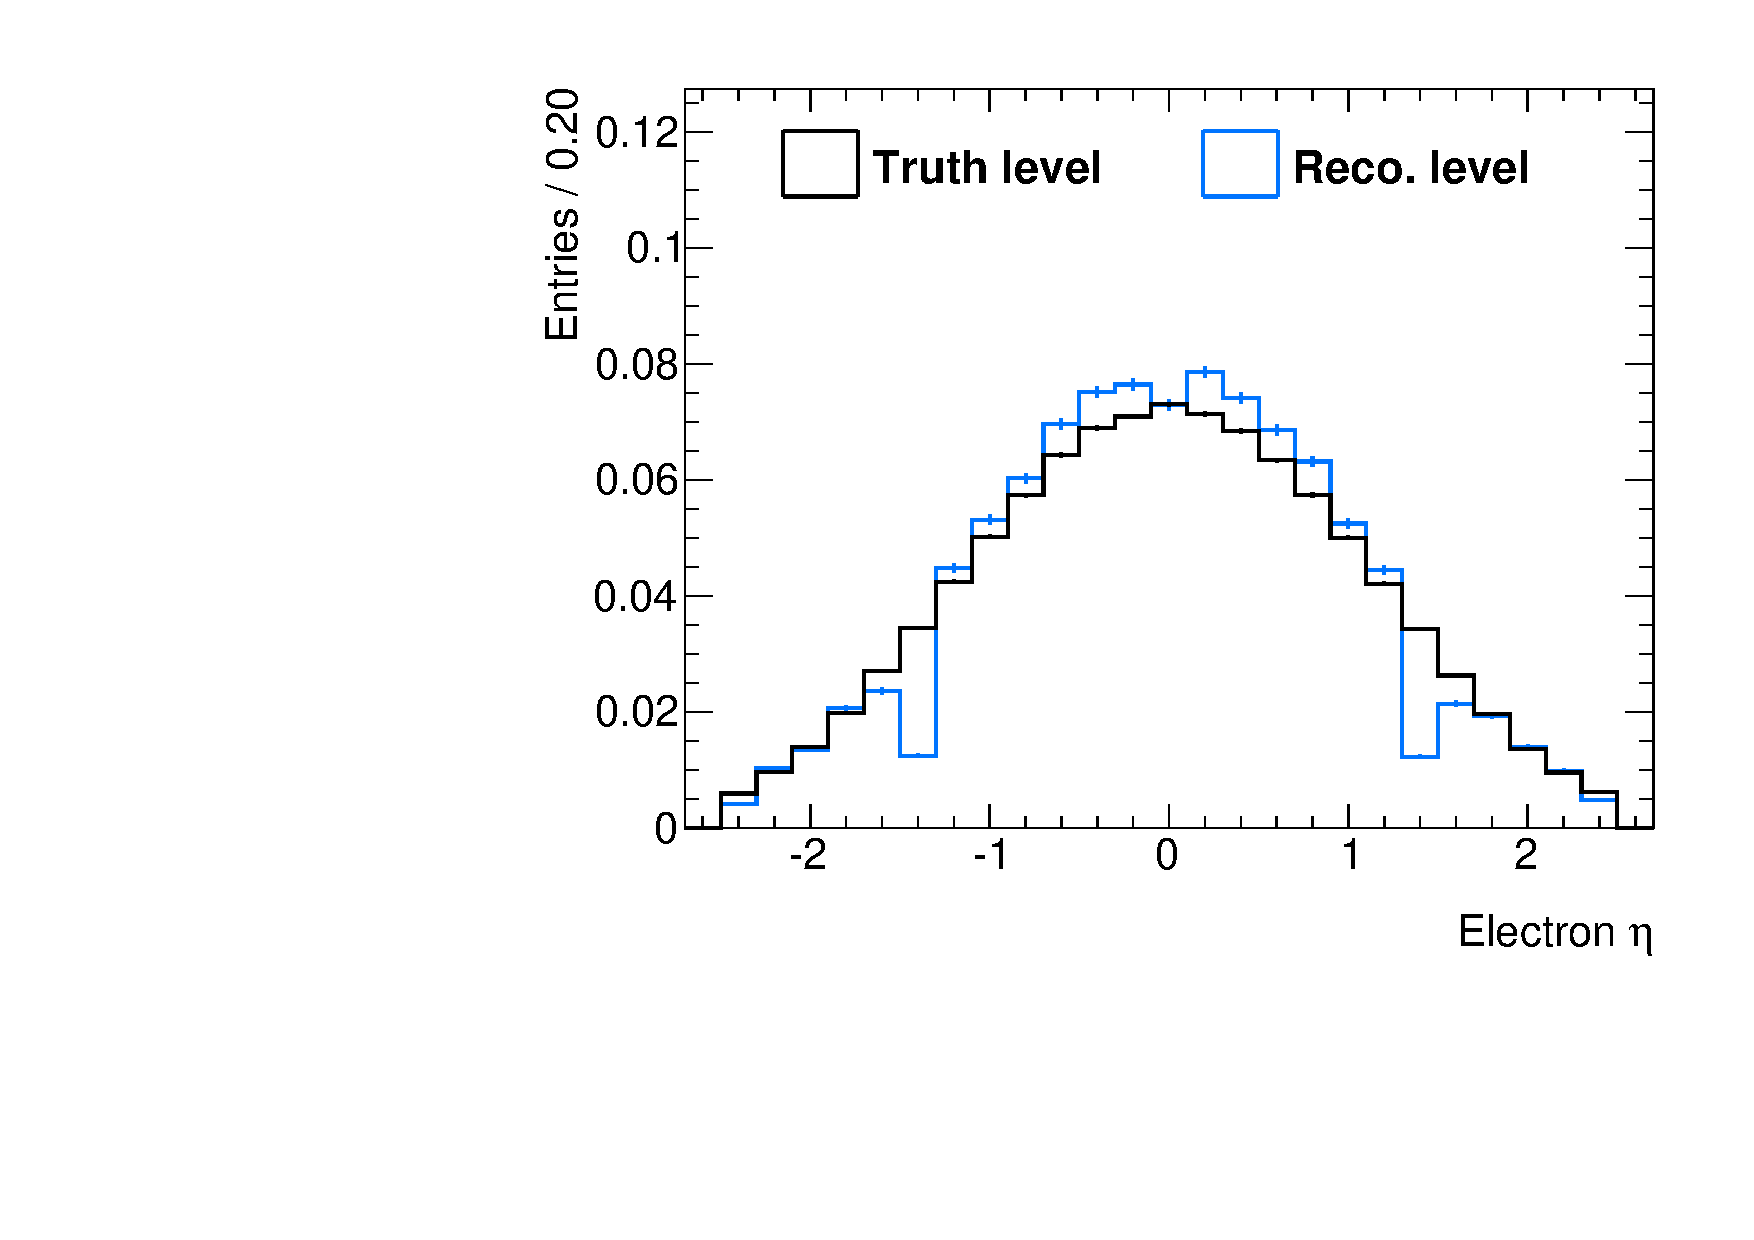
\includegraphics[width=0.49\textwidth]{./figs/fig_8TeV_TRC28_wp70_ptlb130/Dilep_Compare_sel3_recotrue_withtaus_e_Eta.pdf}
  \label{sfig:recotrueeeta}
}
\subfloat[Muon $\eta$]{
  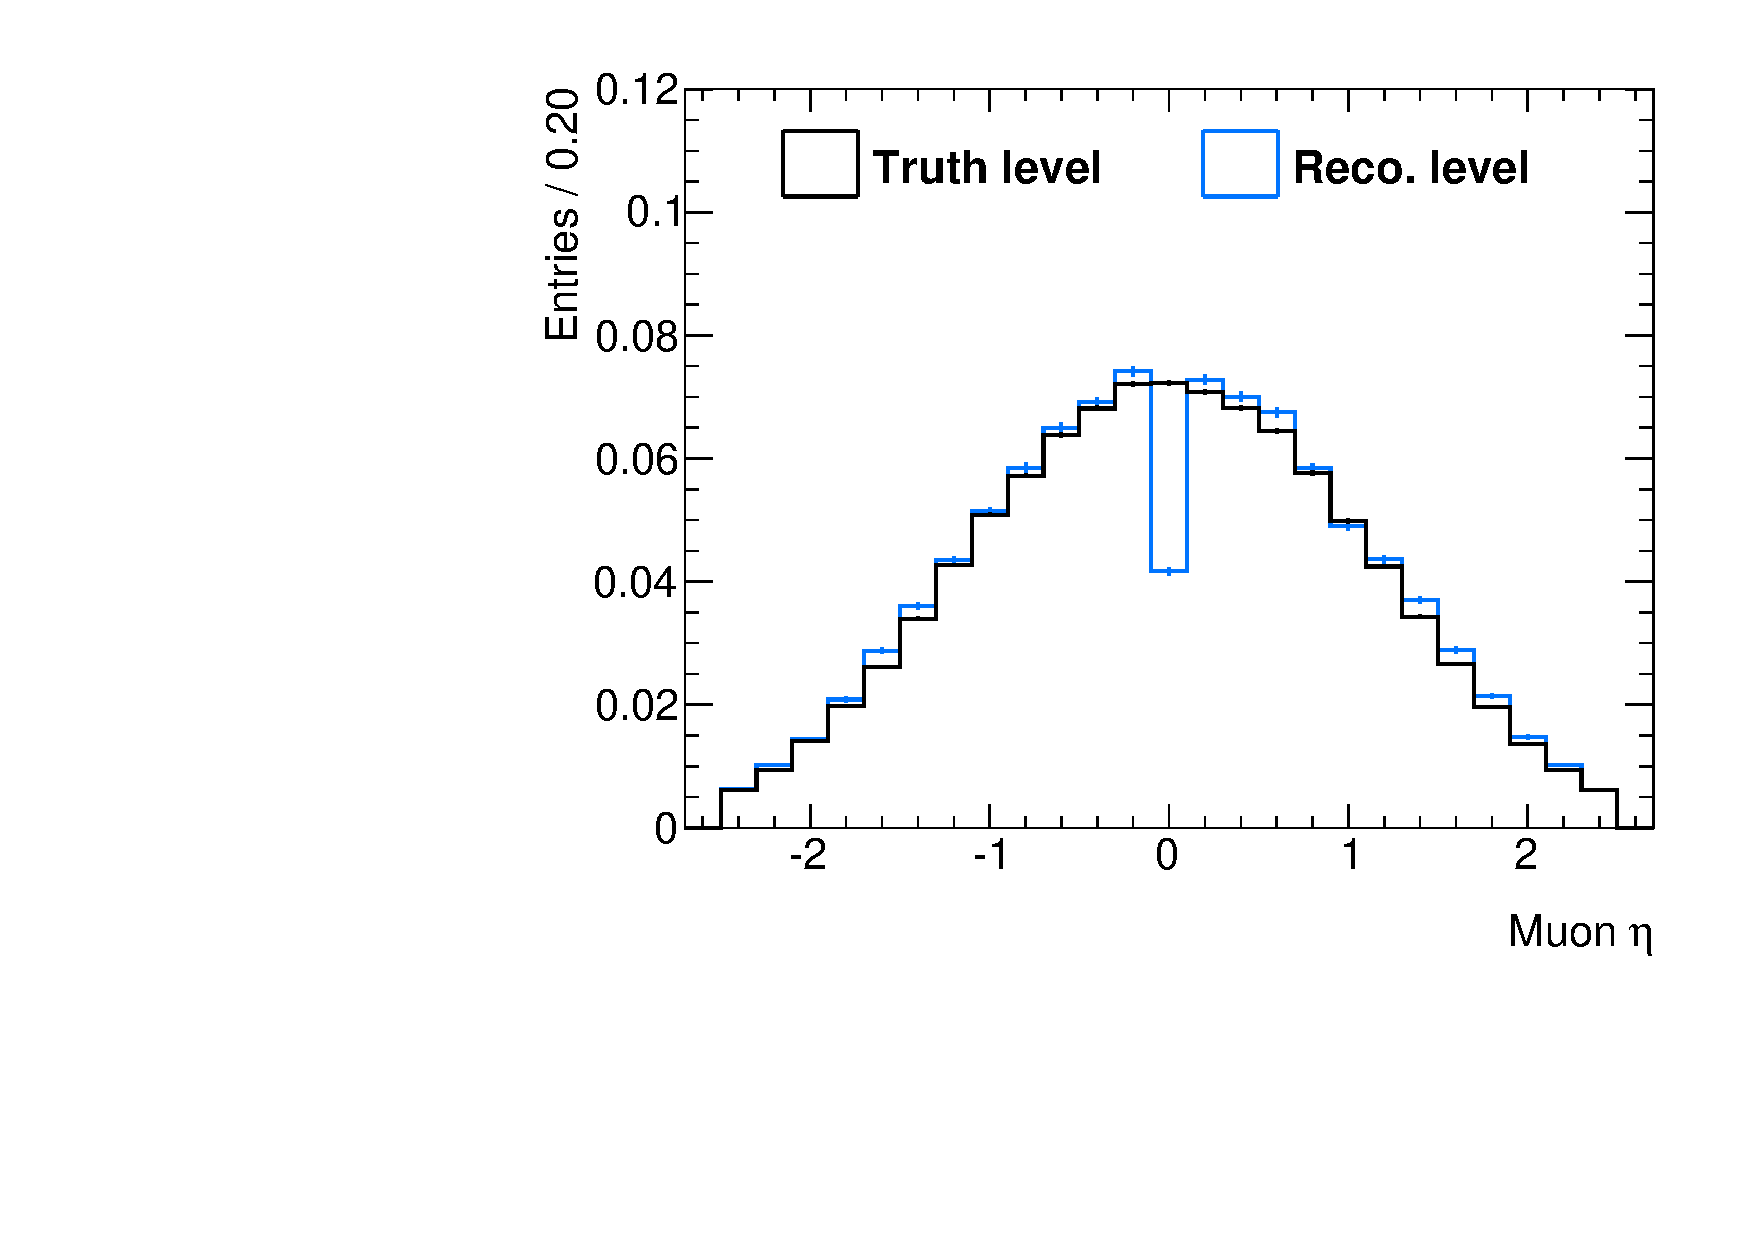
\includegraphics[width=0.49\textwidth]{./figs/fig_8TeV_TRC28_wp70_ptlb130/Dilep_Compare_sel3_recotrue_withtaus_m_Eta.pdf}
  \label{sfig:recotruemeta}
}
\hfill
\subfloat[\mll]{
  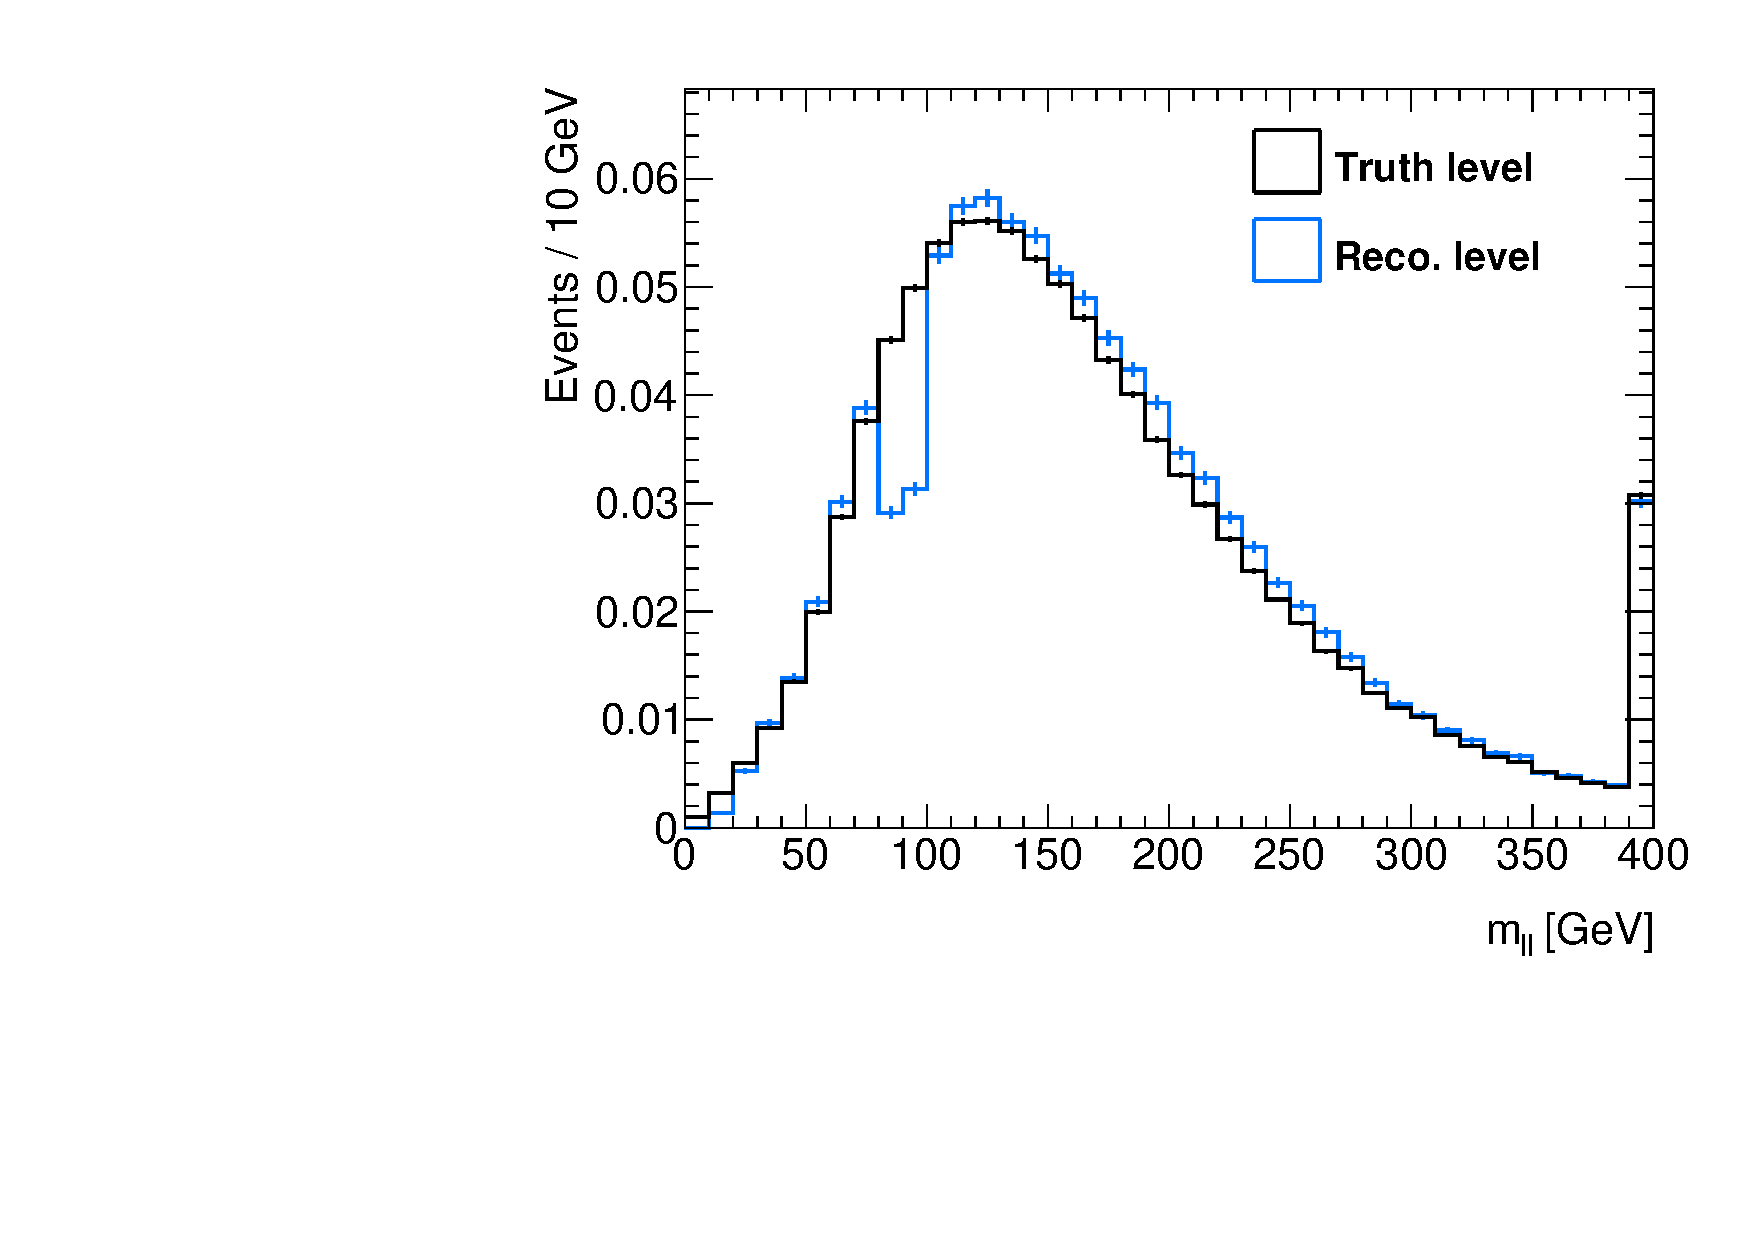
\includegraphics[width=0.49\textwidth]{./figs/fig_8TeV_TRC28_wp70_ptlb130/Dilep_Compare_sel3_recotrue_withtaus_m_ll.pdf}
  \label{sfig:recotruemll}
}
\subfloat[\met]{
  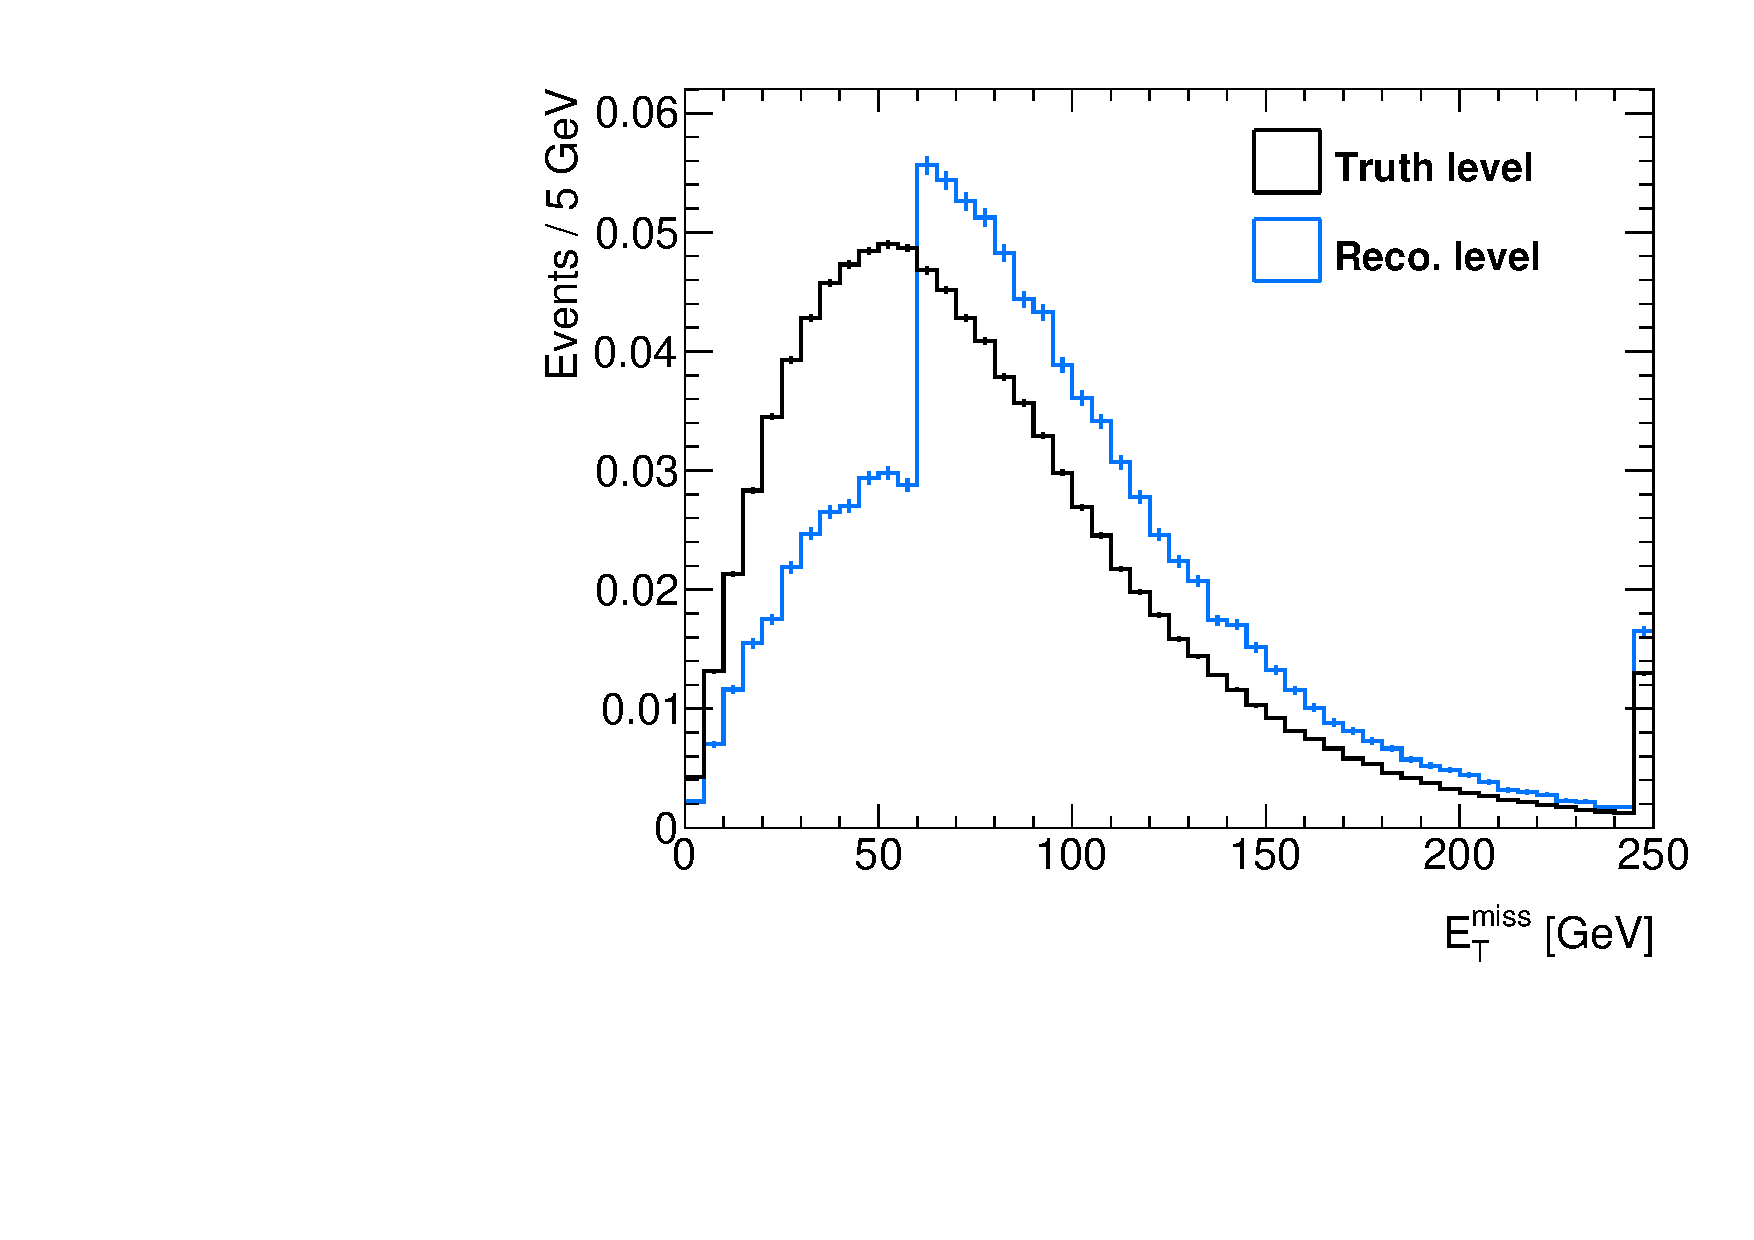
\includegraphics[width=0.49\textwidth]{./figs/fig_8TeV_TRC28_wp70_ptlb130/Dilep_Compare_sel3_recotrue_withtaus_met_et.pdf}
  \label{sfig:recotruemet}
}
\hfill
\subfloat[\ptlb]{
  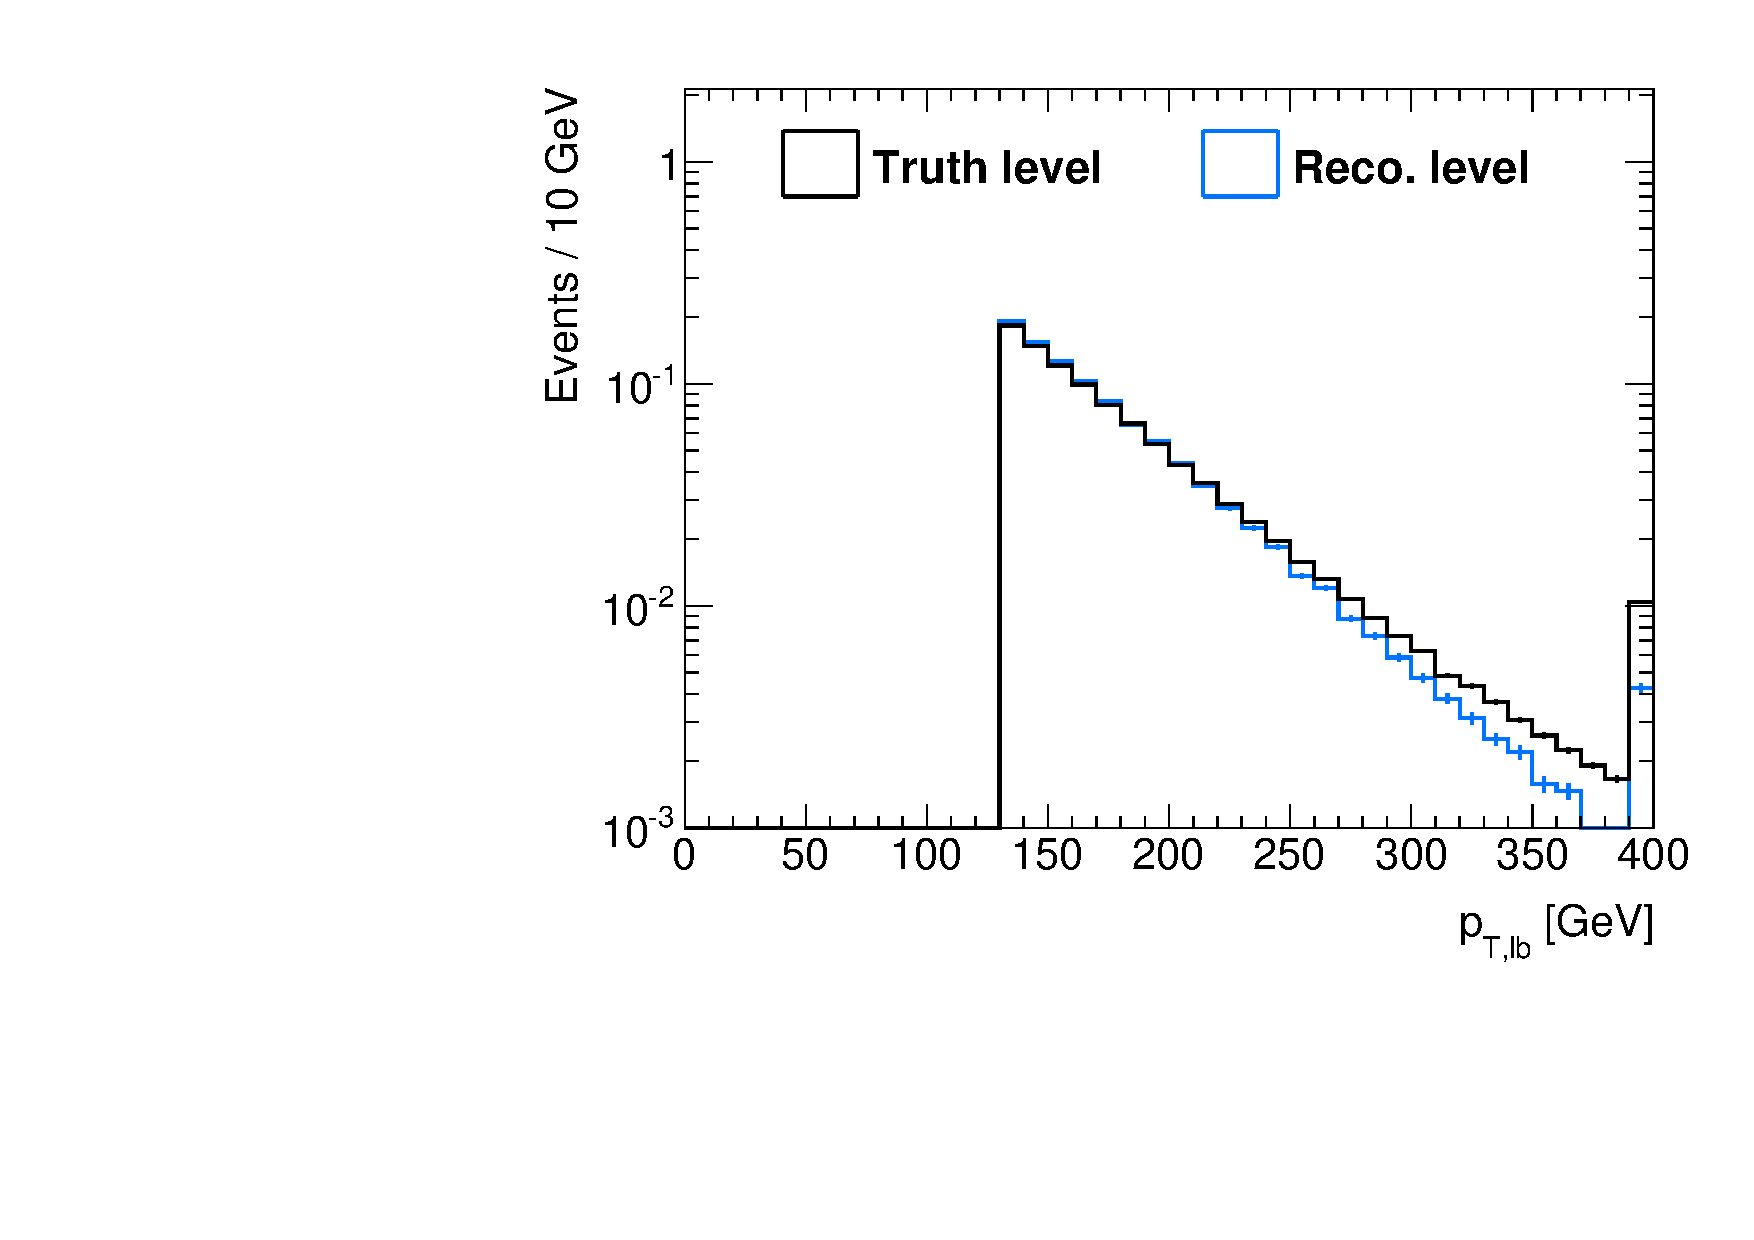
\includegraphics[width=0.49\textwidth]{./figs/fig_8TeV_TRC28_wp70_ptlb130/Dilep_Compare_sel3_recotrue_withtaus_ptlb_logscale.pdf}
  \label{sfig:recotrueptlb}
}
\subfloat[\mlb]{
  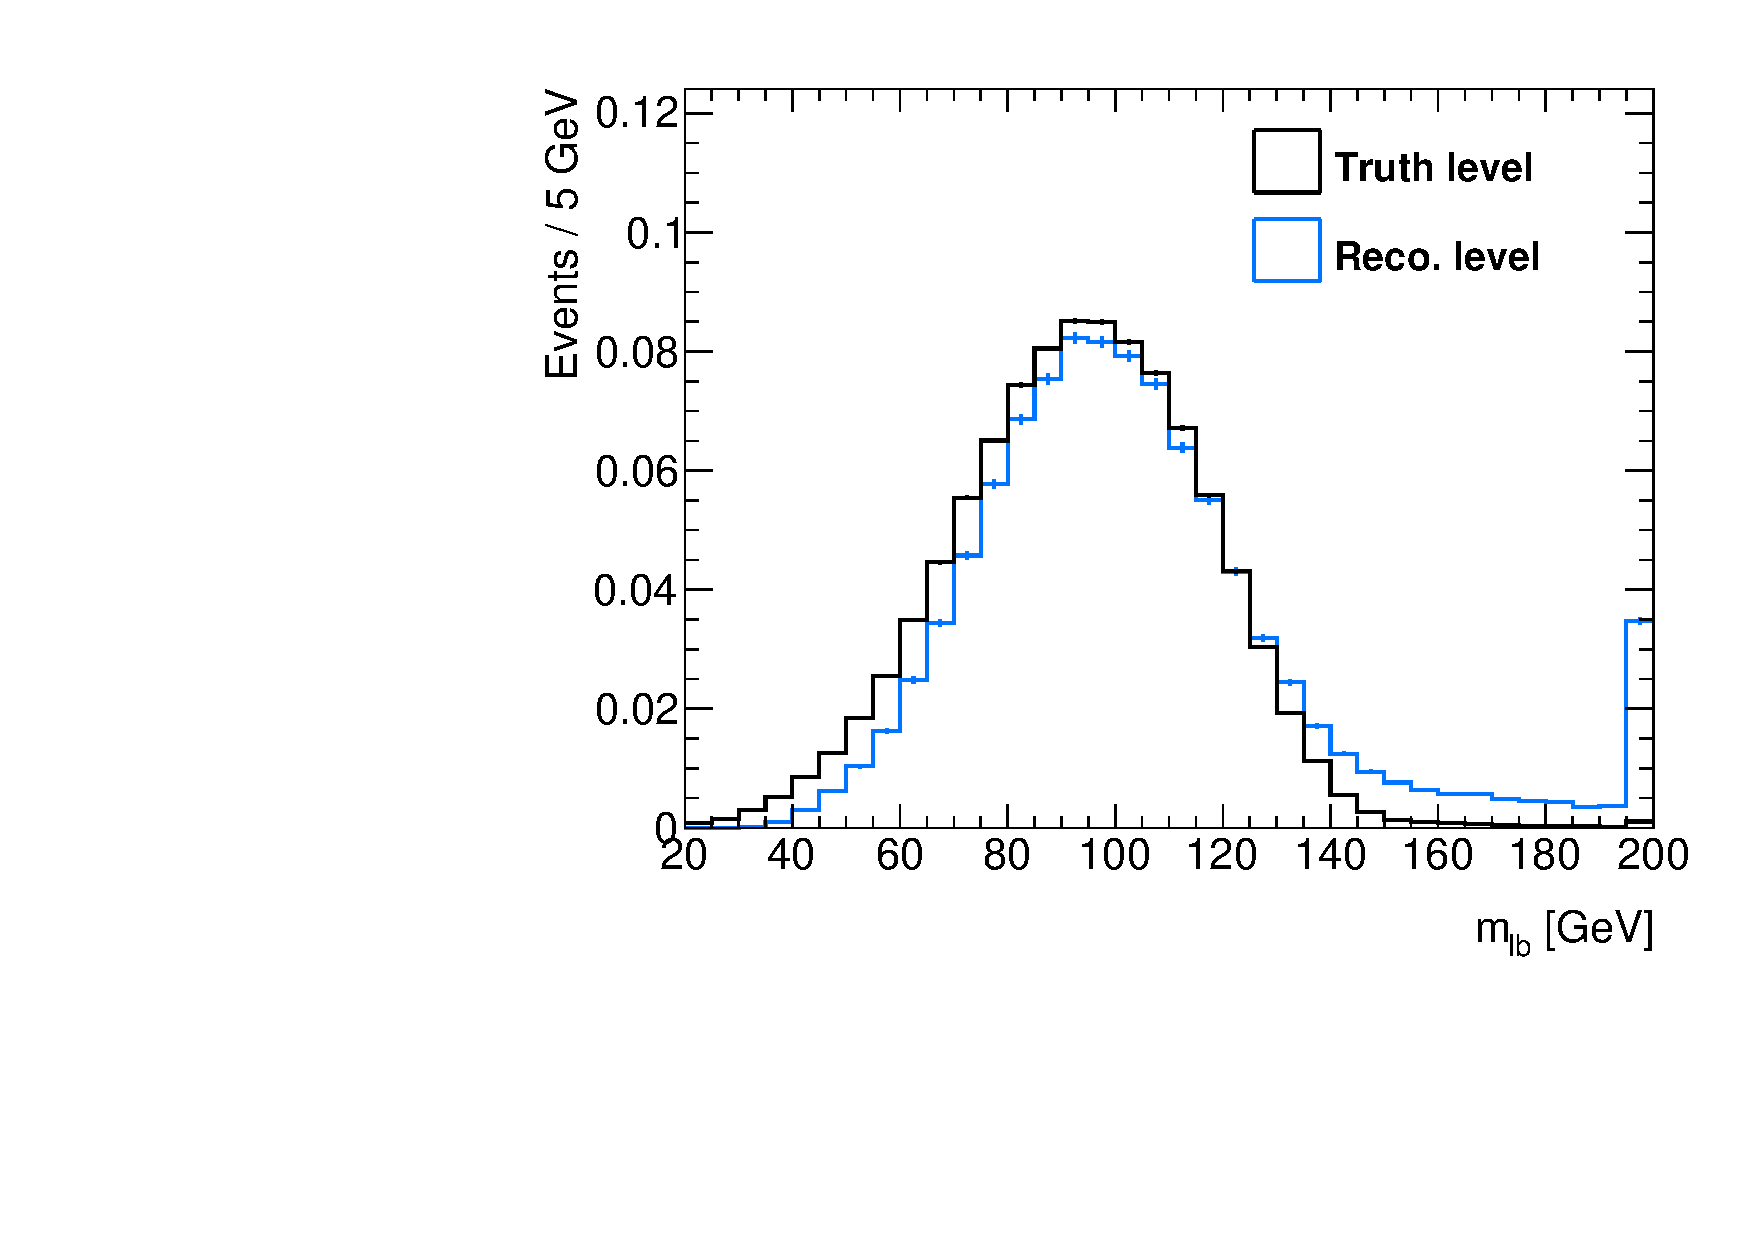
\includegraphics[width=0.49\textwidth]{./figs/fig_8TeV_TRC28_wp70_ptlb130/Dilep_Compare_sel3_recotrue_withtaus_mlb.pdf}
  \label{sfig:recotruemlb}
}
%
\caption[Distributions at \truel\ and \recolevel]{
%
Distributions at \truel\ and \recolevel\ within the fiducial phase space. 
%
\Fig{s}~\subref{sfig:recotrueeeta} and \subref{sfig:recotruemeta} show the electron and muon $\eta$ distributions. 
%
The \mll~\subref{sfig:recotruemll}, the \met~\subref{sfig:recotruemet}, the \ptlb~\subref{sfig:recotrueptlb} and the estimator distribution \mlb~\subref{sfig:recotruemlb} are displayed as well.
%
The uncertainty bars are statistical only, and the rightmost bin contains the overflow, if present.
%
\label{fig:evselrecotrue}
}
\end{figure*}
%%%%%%%%%%%%%%%%%%%%%%%%%%%%%%%%%%%%%%%%%%%%%%%%%%%%%%%%%%%%%%%%%%%%%%%%%%%%%
%
A comparison of normalised \truel\ and \recolevel\ distributions is given in \fig~\ref{fig:evselrecotrue}. 
%
The phase space restrictions, exclusively present at \recolevel, are visible. 
%
\Fig~\subref{sfig:recotrueeeta} displays the effect of the \gls{ECAL} gap on the electron $\eta$ distribution.
%
\Fig~\subref{sfig:recotruemeta} shows the loss of muons at central $\eta$ values due to the reconstruction inefficiency of the \gls{MS}.
%
In \fig{s}~\subref{sfig:recotruemll} and \subref{sfig:recotruemet}, the effect of the \Zboson\ mass and \met\ restrictions in the same lepton flavour channels \ee\ and \mumu\ are visible.
%
\Fig~\subref{sfig:recotrueptlb} shows the \ptlb\ variable which is used for the phase space optimisation. 
%
The estimator distributions \mlb\ at both levels are shown in \fig~\subref{sfig:recotruemlb}. 
%
The \recolevel\ distribution is wider and shifted to larger \mlb\ values.
%
These distributions constitute the basis of the following unfolding procedure.























\subsection{Resolution, binning and regularisation}
%samples
For the training of the unfolding algorithm, the central \ttbar\ \gls{MC} sample with $\mt=172.5$~\GeV\ is used, corresponding to about $\intlumi=360$~\invfb. The corresponding \mlb\ distributions at \recol\ and \truelevel are shown in \fig~\subref*{sfig:recotrue172}.
%
The bin range has been chosen as $\mlb=40$ to $150$~\GeV\ with the outer bins having a width of $35$ and $30$~\GeV\ and the inner bins having a width of $15$~\GeV, resulting in five bins in total. 
%
The regularisation parameter is set to $k=4$.
%
The considerations leading to this decision are detailed in the following.
%
%%%%%%%%%%%%%%%%%%%%%%%%%%%%%%%%%%%%%%%%%%%%%%%%%%%%%%%%%%%%%%%%%%%%%%%%%%%%%%%
\begin{figure*}[tbp!]
\centering
\subfloat[\mlb\ for $\mt=172.5$~\GeV]{
  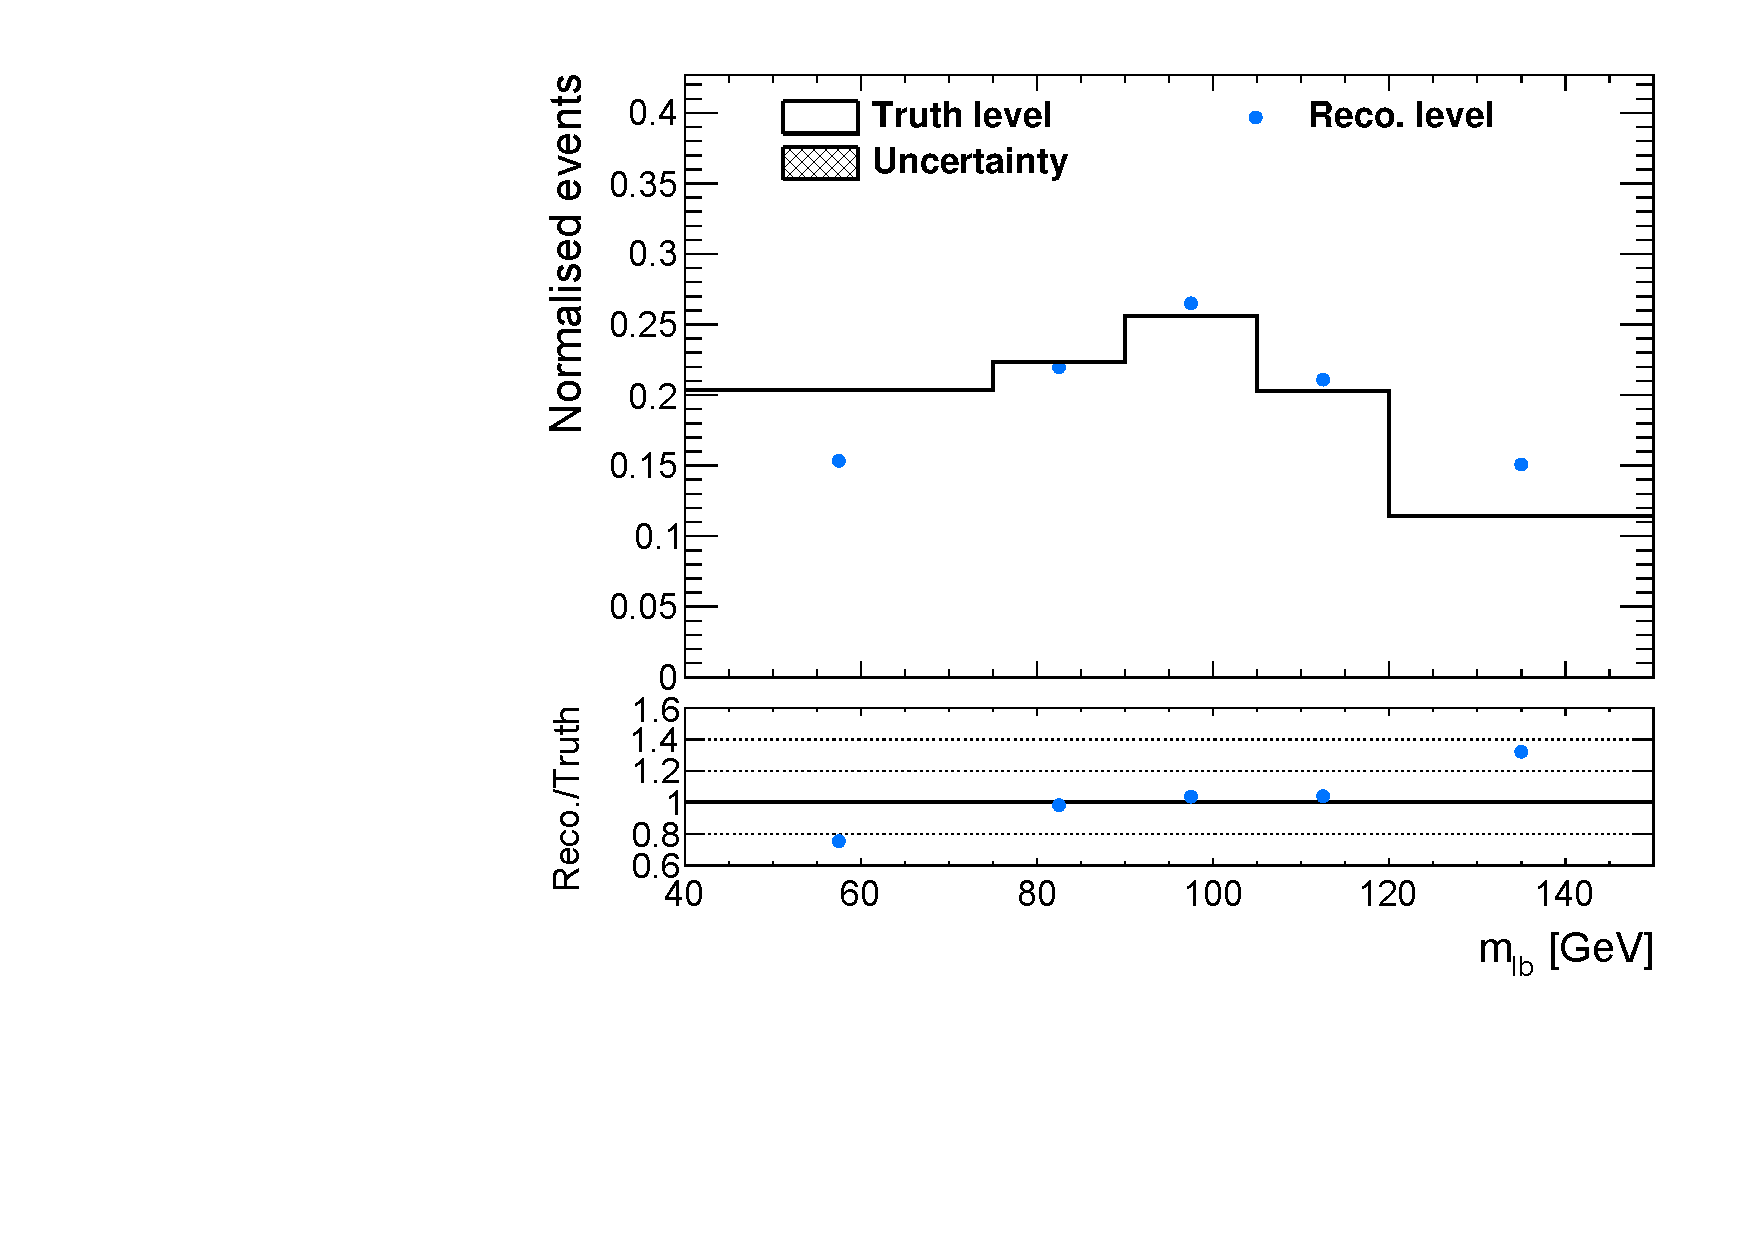
\includegraphics[width=0.49\textwidth]{./figs/fig_8TeV_TRC28_wp70_unfolding_ptlb130/mlb_unfold_hl_5bins_large_SVD_4_recotrue.pdf}
  \label{sfig:recotrue172}
}
\subfloat[Total \mlb\ response]{
  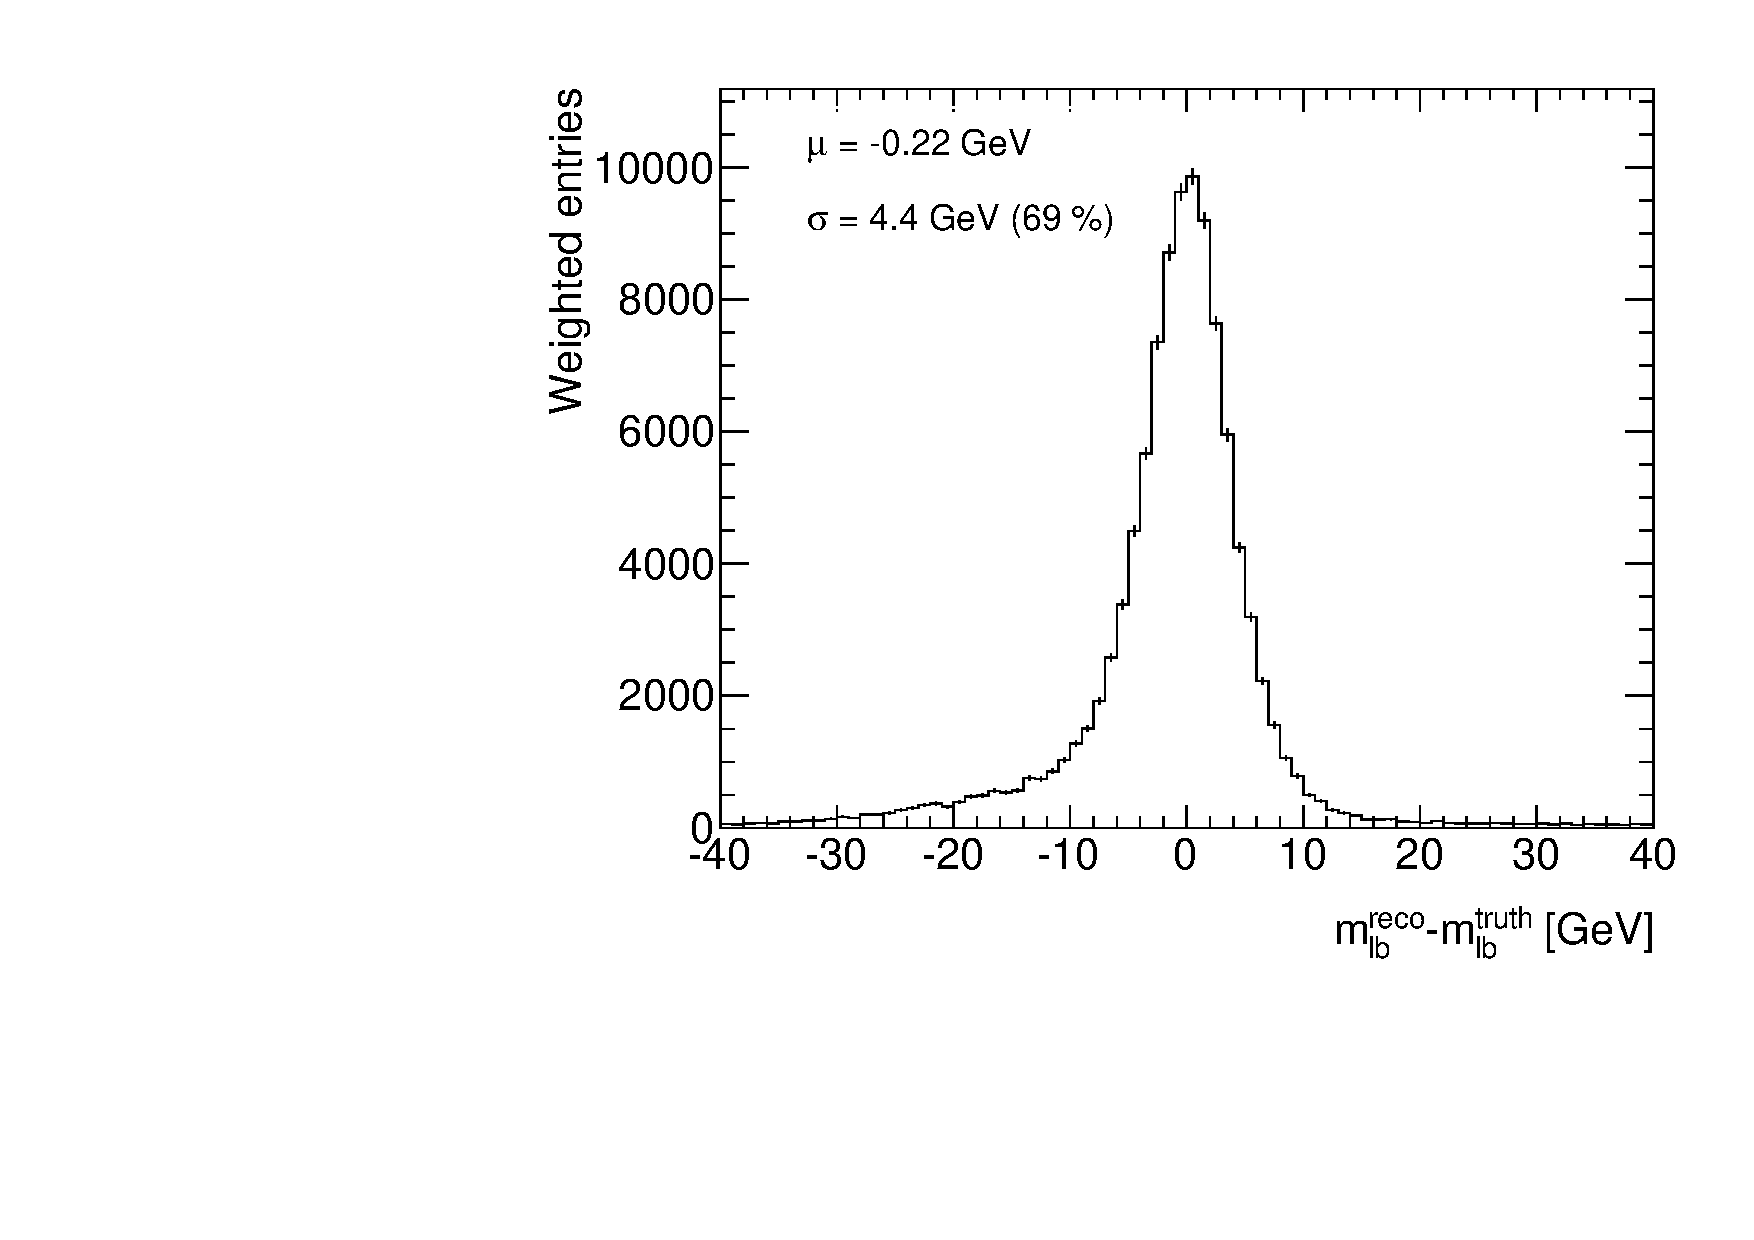
\includegraphics[width=0.49\textwidth]{./figs/fig_8TeV_TRC28_wp70_unfolding_ptlb130/mlb_unfold_hl_5bins_large_SVD_4_resolution.pdf}
  \label{sfig:unfoldres}
}
\hfill
\subfloat[Resolution profile]{
  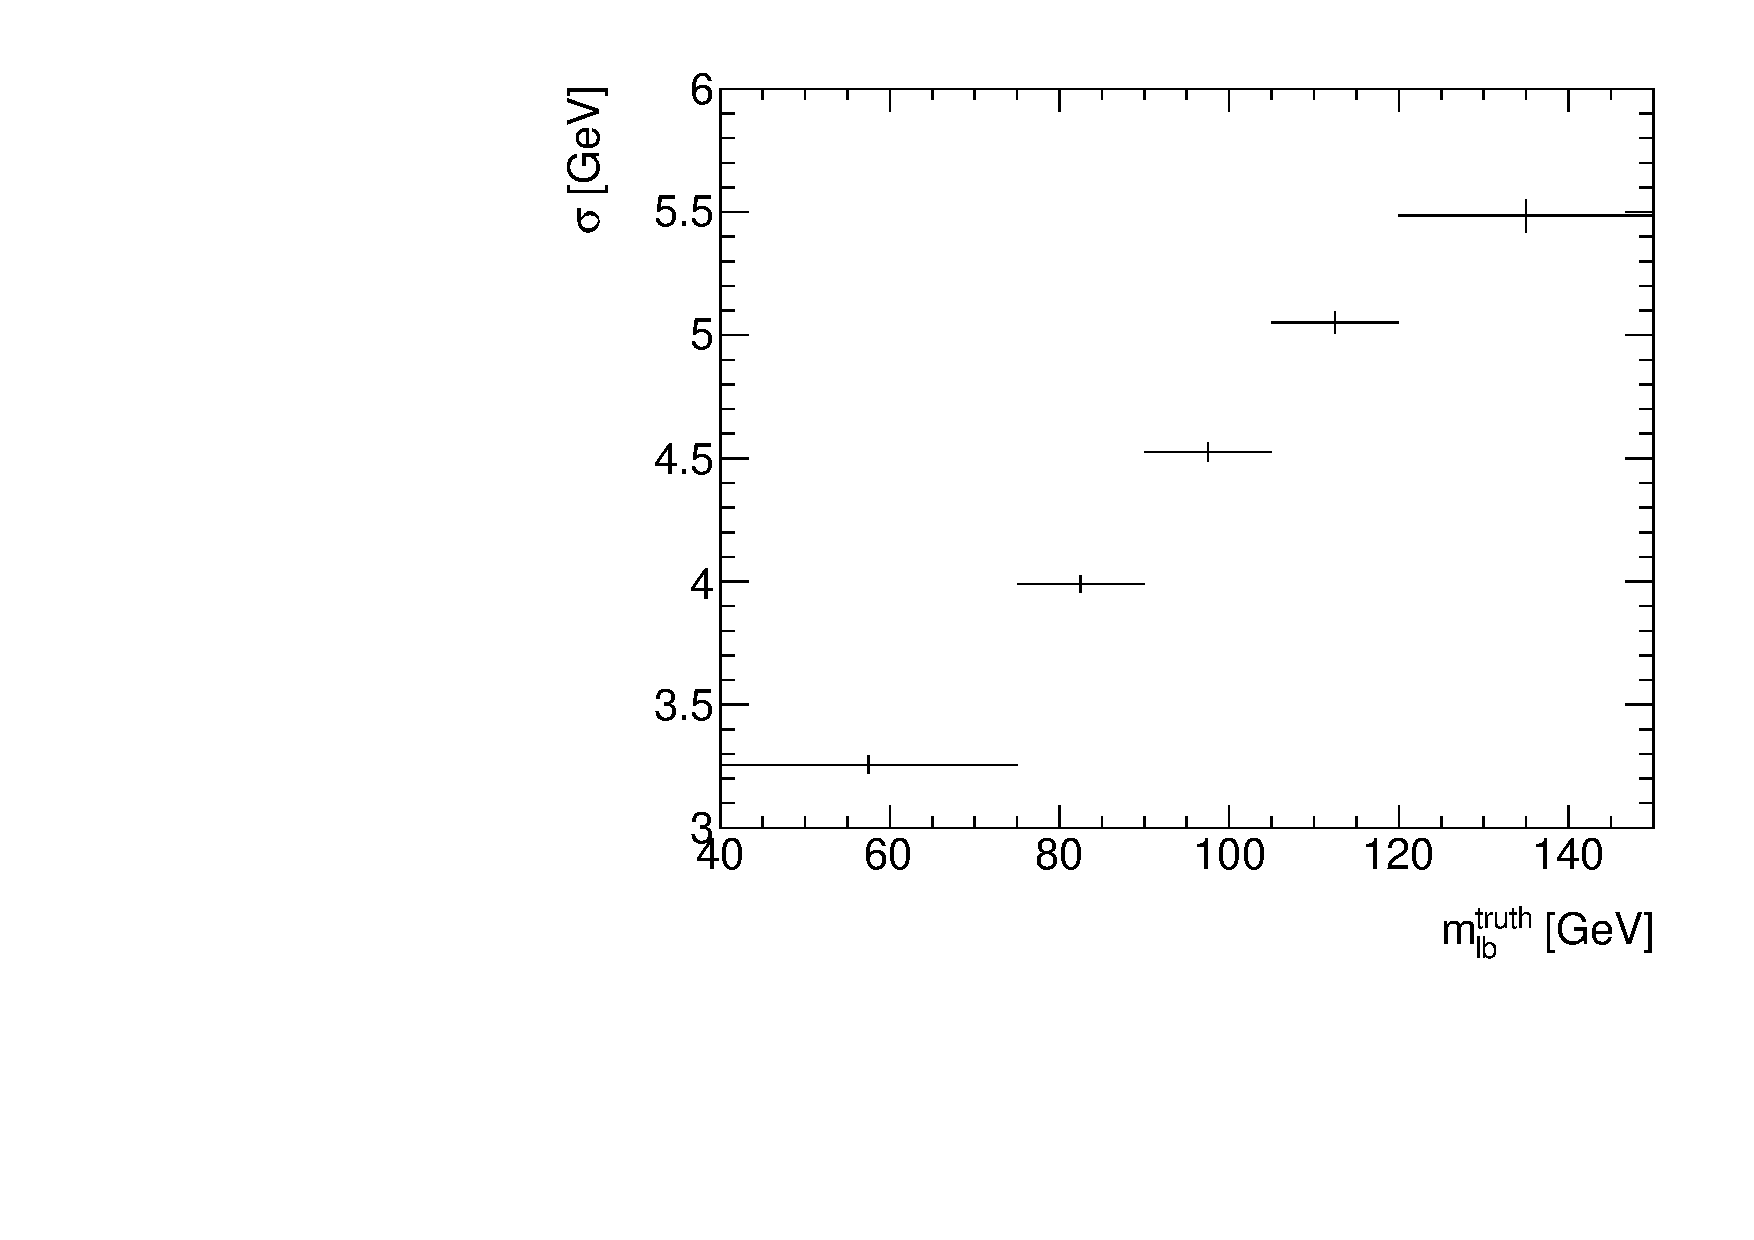
\includegraphics[width=0.49\textwidth]{./figs/fig_8TeV_TRC28_wp70_unfolding_ptlb130/mlb_unfold_hl_5bins_large_SVD_4_res_profile.pdf}
  \label{sfig:unfoldresprofile}
}
\subfloat[Bin migration matrix $\mathbf{M}$]{
  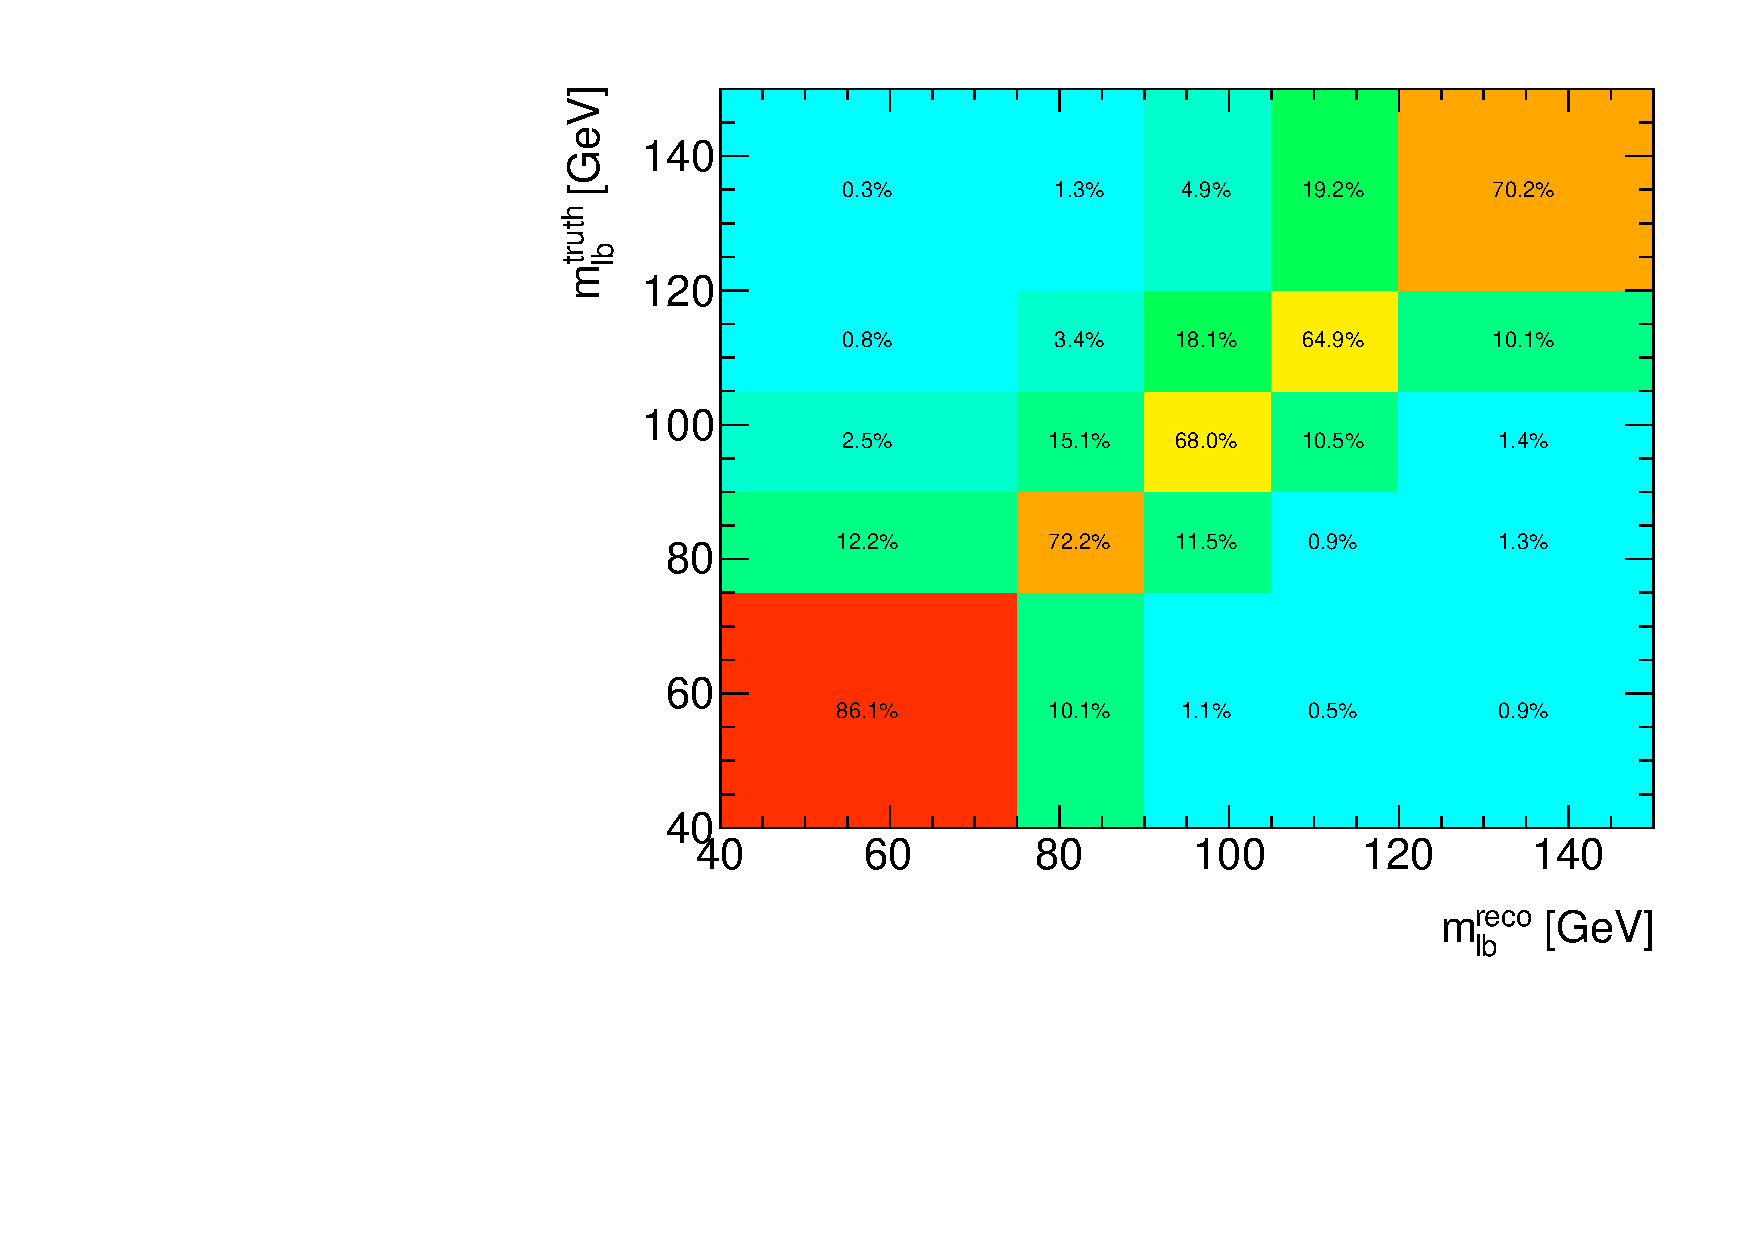
\includegraphics[width=0.49\textwidth]{./figs/fig_8TeV_TRC28_wp70_unfolding_ptlb130/mlb_unfold_hl_5bins_large_SVD_4_migration.pdf}
  \label{sfig:migrationmatrix}
}
\hfill
\subfloat[Response matrix $\mathbf{R}$]{
  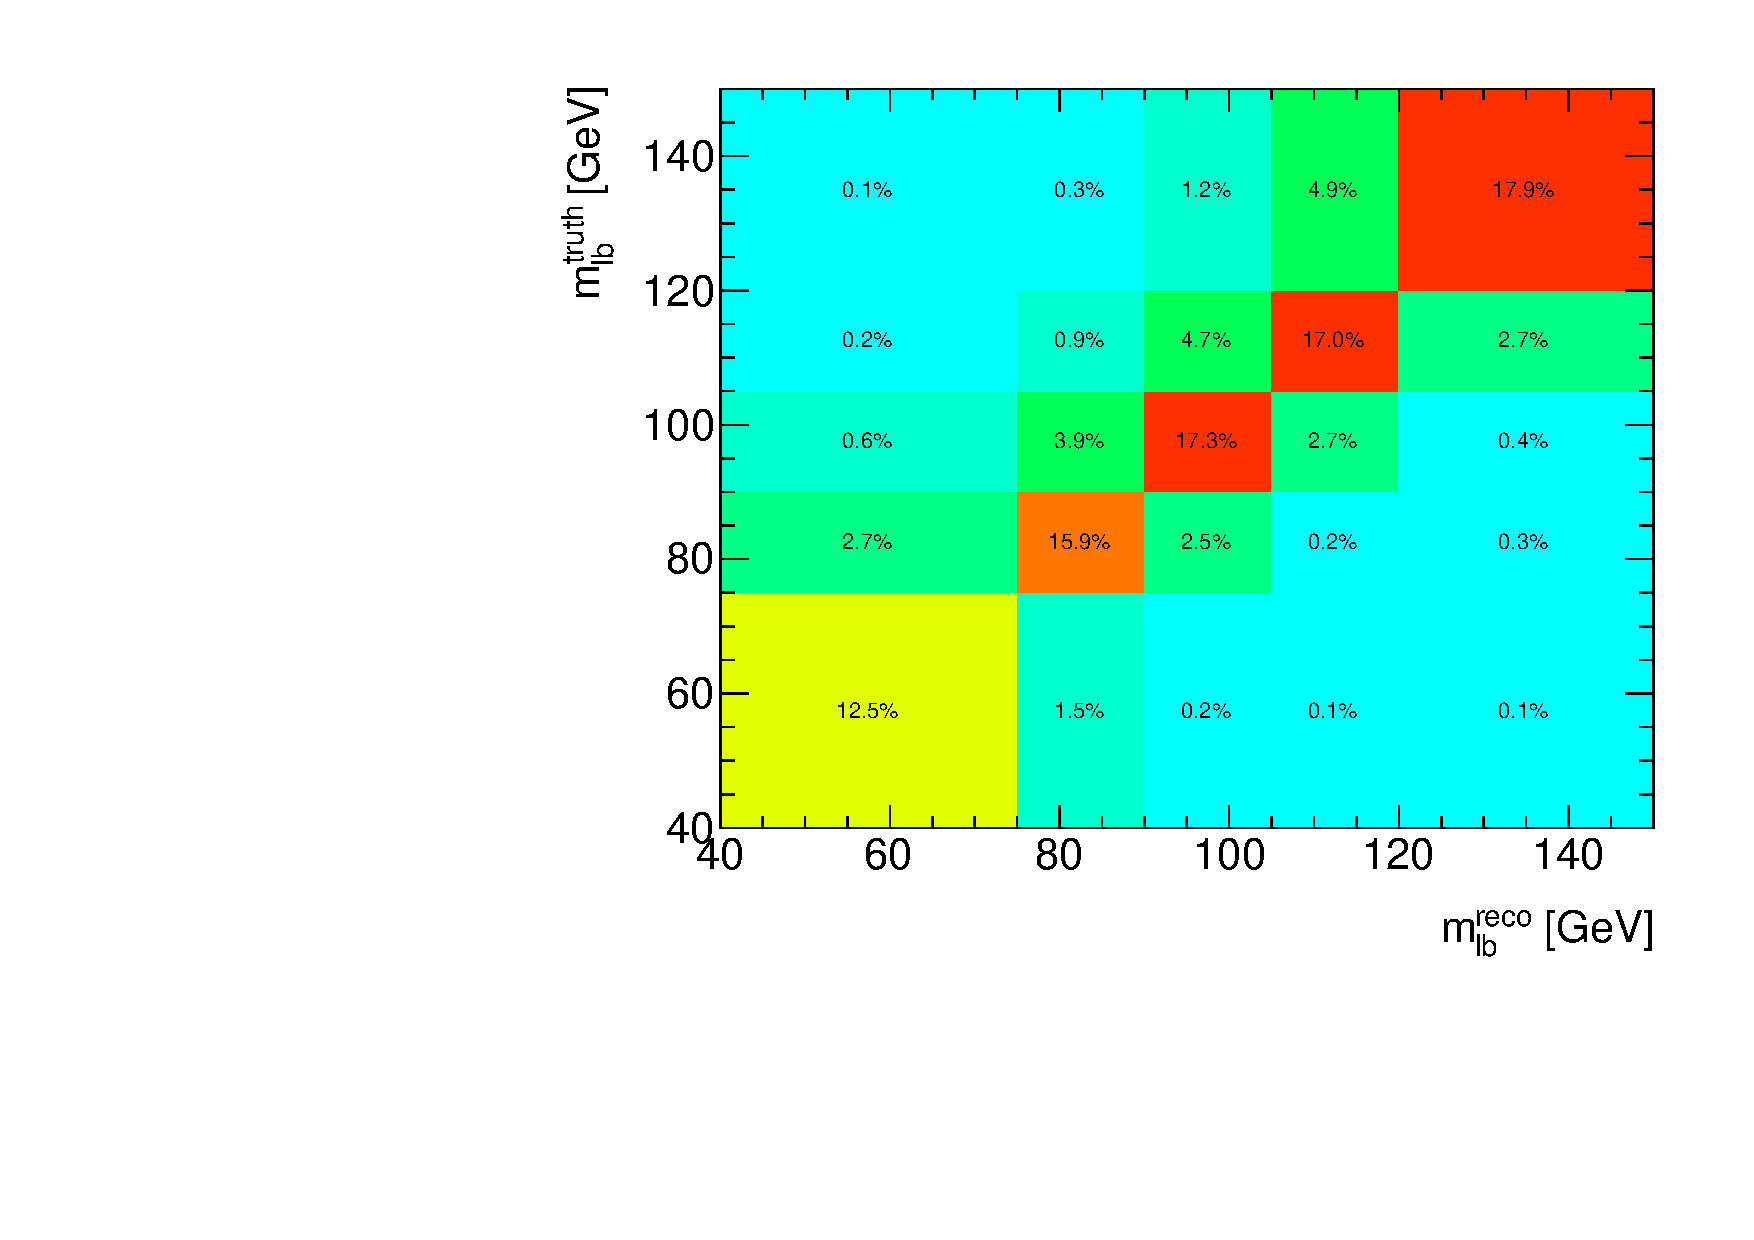
\includegraphics[width=0.49\textwidth]{./figs/fig_8TeV_TRC28_wp70_unfolding_ptlb130/mlb_unfold_hl_5bins_large_SVD_4_response.pdf}
  \label{sfig:responsematrix}
}
\caption[Resolution and response for unfolding]{
%
\Fig~\subref{sfig:recotrue172} shows the normalised \mlb\ distributions at \recol\ and \truelevel\ for $\mt=172.5$~\GeV, which are used to determine the response matrix $\mathbf{R}$.
%
%
\Fig~\subref{sfig:unfoldres} shows the residual distribution of the \recol\ and \truelevel\ \mlb\ values and \subref{sfig:unfoldresprofile} the change of its width $\sigma$ as a function of \mlbt. Each width is taken from a fit of a Gaussian function to the peak of the \mlb\ residual distribution.
%
\Fig{s}~\subref{sfig:migrationmatrix} and \subref{sfig:responsematrix} show the bin migration matrix $\mathbf{M}$ and the response matrix $\mathbf{R}$ for the chosen binning. In each bin, the percentage of bin entries corresponding to a given \mlbt\ value resulting in the respective \mlbr\ bin is given.
%
\label{fig:unfoldresolution}
}
\end{figure*}
%%%%%%%%%%%%%%%%%%%%%%%%%%%%%%%%%%%%%%%%%%%%%%%%%%%%%%%%%%%%%%%%%%%%%%%%%%%%%
%



Low values of $k$ bias the unfolded distribution towards the training distribution, while high parameter values make it susceptible to statistical fluctuations. All parameter values of $k$ between 1 and the number of bins have been tested and the unfolded distribution has been compared to the underlying truth distribution. Parameter values around half the number of bins yield comparable performance in terms of compatibility of the unfolded distribution with the underlying \truelevel\ distribution.


The event by event difference of the estimator values at truth and \recolevel\ is shown in \fig~\subref*{sfig:unfoldres}. As expected from the \mlb\ distribution shapes in \fig~\subref*{sfig:recotruemlb}, the \mlb\ response is slightly asymmetric and biased towards larger \mlbr\ values. A fit of a Gaussian function to the peak of the response distribution ($\vert\mlbr-\mlbt\vert<10$~\GeV) is taken as an approximation of the average bias and the resolution from the Gaussian $\mu$ and $\sigma$ parameters, resulting in a bias of about \averagebias\ and a resolution of about \averageres. The region $\mu\pm\sigma$ contains \eventsinpeak\ of all events. 
%
The resolution changes as a function of \mlbt, as shown in \fig~\subref*{sfig:unfoldresprofile}. To minimise bin migration effects due to resolution, i.e. the off-diagonal elements of the bin migration matrix $\mathbf{M}$, the bin widths for the unfolding have been chosen well above twice the resolution, leading to a minimum bin width of about $\Delta\mlb=15$~\GeV.
%
\Fig~\subref*{sfig:migrationmatrix} shows $\mathbf{M}$ as the percentage of bin entries of a given \mlbt\ value in the respective \mlbr\ bin. The probability for a given event at \truelevel\ to be reconstructed in the same bin at \recolevel\ is therefore given on the diagonal, while the off-diagonal elements represent the probability of migration to another bin. By construction, the numbers per row add up to $100\%$.
%
% For too fine bin widths, the bin to bin migrations are large, resulting in large off-diagonal elements in the response matrix and inter-bin correlations in the unfolded histogram, complicating a comparison to theory predictions. This can be avoided by the choice of a bin width resulting in a close to diagonal migration matrix.
% %
While the diagonal elements show entries well above $60\%$, the migrations between neighbouring bins range from about $10\%$ to $20\%$. A finer binning would increase this bin migration and further complicate the unfolding procedure.
%
To avoid complications from bins with low statistics, the bin range and width are chosen to exclude or merge sparsely populated bins. This, together with the correlation argument, leads to the decision of larger outer bin widths.


However, the most important criterion for the choice of binning and regularisation is the performance of the unfolding algorithm described next.
%
%  in terms of the reproduction of \truelevel\ distributions and of the consistent assignment of uncertainties. This also includes the performance of the fit method, applied to assess the value of \mt\ at \truelevel.
% %
% This criterion led to the particular bin and regularisation parameter choice from the various combinations satisfying the aforementioned criteria. 
% %
% These investigations are detailed together with the assessment of the fit performance in \sect~\ref{sect:unfoldsyst}.


















\subsection{Unfolding and closure tests}
%https://cds.cern.ch/record/1647176/files/ATL-COM-PHYS-2014-086.pdf
Using the parameter settings determined in the previous section, the unfolding method is trained, using the central \ttbar\ sample. 
%
Taking into account the inefficiency and fake contributions, the response matrix $\mathbf{R}$ in \fig~\subref*{sfig:responsematrix} is derived. 
%
The \gls{SVD} technique is used to invert the matrix.
%
%%%%%%%%%%%%%%%%%%%%%%%%%%%%%%%%%%%%%%%%%%%%%%%%%%%%%%%%%%%%%%%%%%%%%%%%%%%%%%%
\begin{figure*}[tbp!]
\centering
\subfloat[$\mt=170$~\GeV]{
	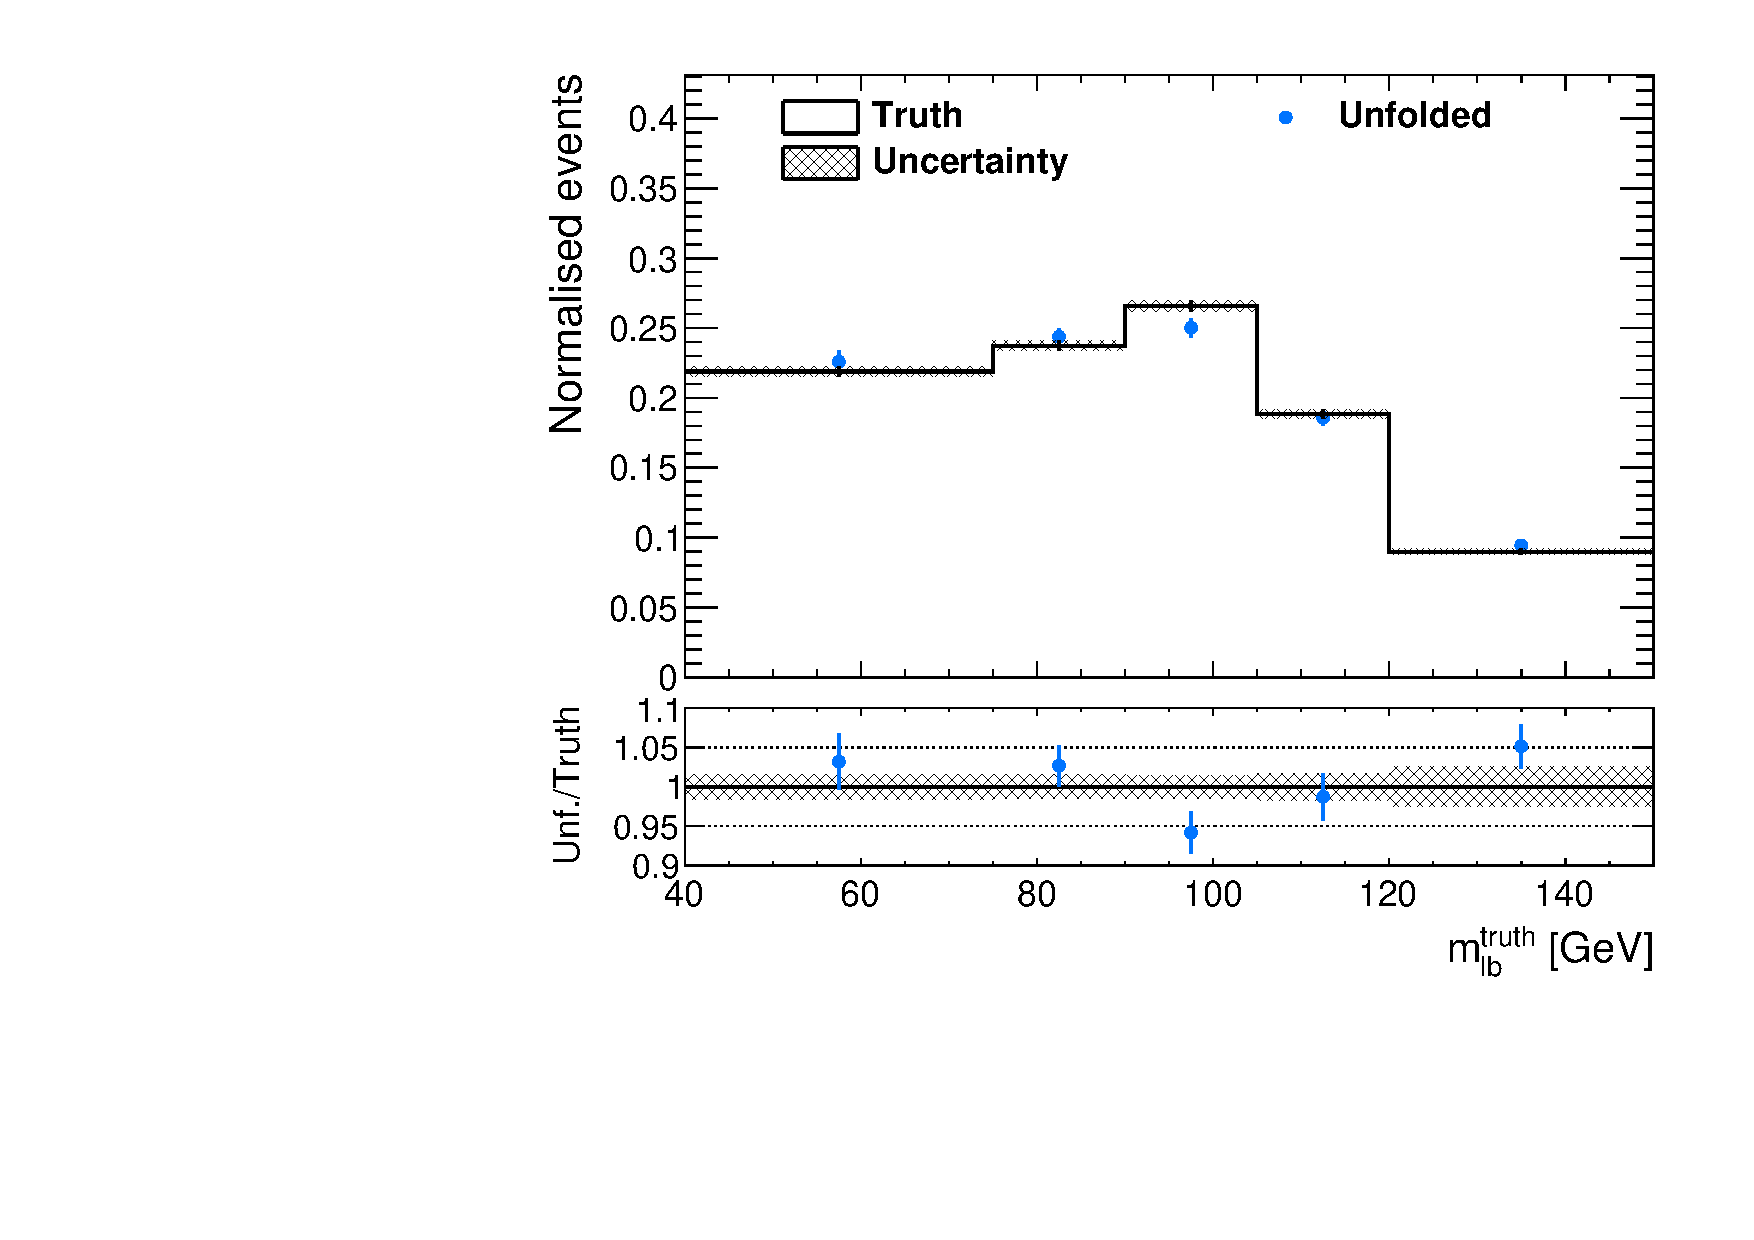
\includegraphics[width=0.49\textwidth]{{./figs/fig_8TeV_TRC28_wp70_unfolding_ptlb130/mlb_unfold_hl_5bins_large_SVD_4_unftesttrue.closure170}.pdf}
  \label{sfig:closure170}
}
\subfloat[$\mt=175$~\GeV]{
	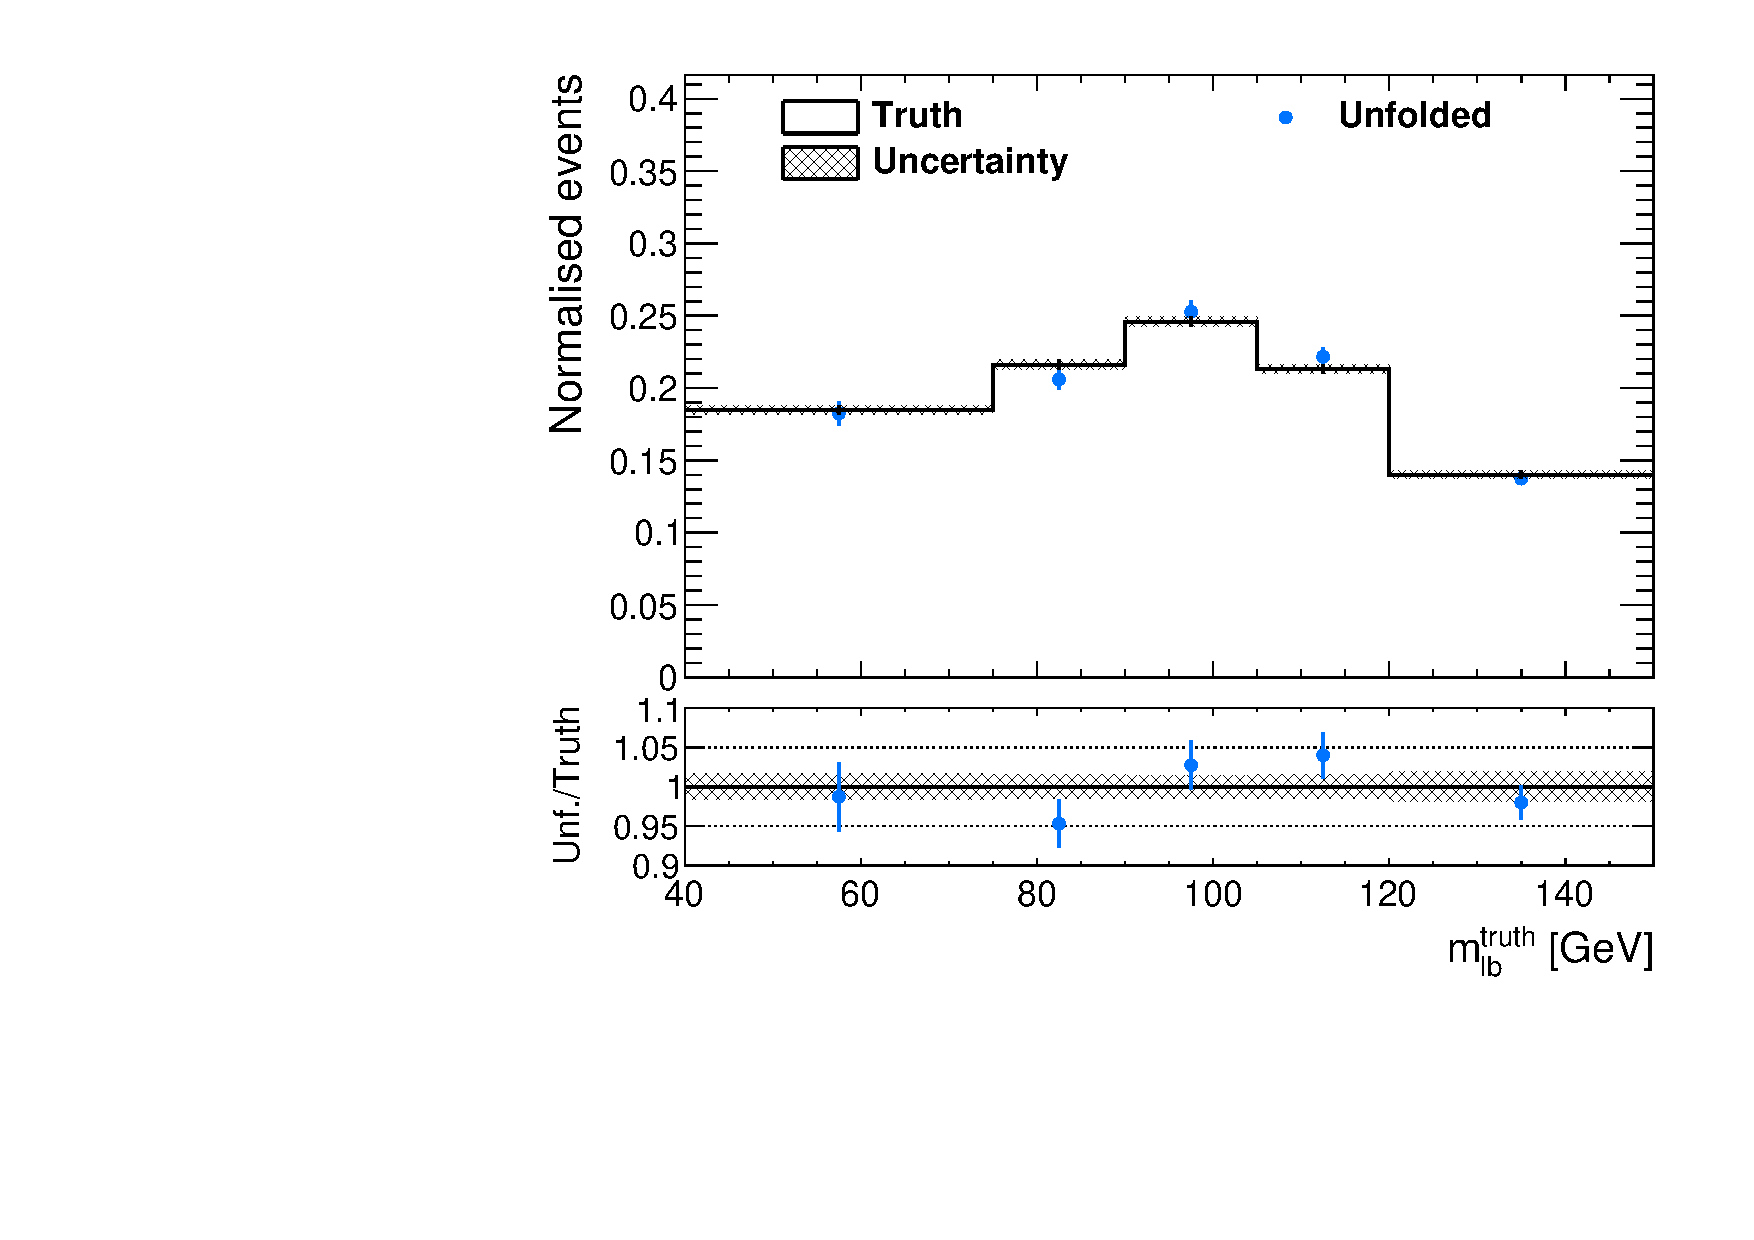
\includegraphics[width=0.49\textwidth]{{./figs/fig_8TeV_TRC28_wp70_unfolding_ptlb130/mlb_unfold_hl_5bins_large_SVD_4_unftesttrue.closure175}.pdf}
  \label{sfig:closure175}
}
\caption[Unfolded \mlb\ \gls{MC} distributions]{
%
The unfolded \mlbr\ distributions at \subref{sfig:closure170} $\mt=170$ and \subref{sfig:closure175} $175$~\GeV\ using the response matrix obtained from the sample at $\mt=172.5$~\GeV\ in comparison to their underlying \truelevel\ distribution. 
%
The histograms are statistically independent, since they are derived from disjunct subsets of the full \gls{MC} sample.
%
The bins of the unfolded histogram are correlated and the uncertainty corresponding uncertainty band includes the uncertainties due to statistics and the unfolding procedure.
%
The bins of the \truelevel\ templates are uncorrelated and the uncertainty bars are statistical only.
%
Taking into account the bin correlation from the unfolding procedure, the \truel\ and unfolded level histograms agree with \chidof\ values of 8.1/4 and 5.5/4, corresponding to probabilities of 8.8 and 24\%, respectively.
%
\label{fig:unfoldclosure}
}
\end{figure*}
%%%%%%%%%%%%%%%%%%%%%%%%%%%%%%%%%%%%%%%%%%%%%%%%%%%%%%%%%%%%%%%%%%%%%%%%%%%%%



%closure
The performance of the determined response matrix is tested, using the statistically independent templates at the neighbouring \tquark\ mass points $\mt=170$ and $175$~\GeV. To avoid correlation between the unfolded result and the corresponding \truelevel\ distribution, these samples are split into two parts, 80\% to be used at \recolevel\ for the unfolding and 20\% to be used at \truelevel\ to obtain statistically independent distributions for consistency tests. 
%
The response matrix $\mathbf{R}$ is kept fixed to the one determined from the full $\mt=172.5$~\GeV\ \gls{MC} sample.
%
The unfolded in comparison to the \truelevel\ distributions is shown in \fig{s}~\subref*{sfig:closure170} and \subref*{sfig:closure175}. For each \mt\ value, the \chiq\ value divided by the \gls{ndf} shows that the unfolded distribution is in good agreement with the \truelevel\ distribution. The \chiq\ is calculated taking into account the covariance matrix of the unfolded result, with the variances of the \truelevel\ histogram added to the diagonal. 
%
The relative size of the variances due to the sample statistics with respect to the variances due to the unfolding procedure amounts to about $20\%$ in the rightmost and about $5\%$ in the other bins.
%
% The same capability of reproducing the underlying \truelevel\ distribution has been observed in 1000 pseudo-experiments from unfolding randomly varied data-sized \recolevel\ distributions.
%
% As an additional investigation, 1000 pseudo-experiments are drawn from both samples, each constructed by randomly drawing events, passing either the \recolevel, the \truelevel\ or both event selections, until an integrated \recolevel\ event weight equal to the number of expected data events has been reached. This procedure ensures the correct contribution of fake and inefficiency events. 
% %
% These distributions are unfolded and the resulting histograms are then compared to the respective \truelevel\ histograms. The residual distributions of the histogram mean and \gls{RMS} are Gaussian distributed and yield an average bias of \closureaveragebiasbelow\ (\closureaveragebiasabove)~\GeV\ and an \gls{RMS} deviation of \closureaveragewidthbelow\ (\closureaveragewidthabove)~\GeV\ for $\mt=170$ ($175$)~\GeV.  This bias is consistent with zero and the increase of the width indicates the loss of resolution by the unfolding procedure. The impact in terms of \mt\ is evaluated in \sect~\ref{sect:unfoldsyst}.

Altogether, this shows that the unfolding procedure returns the underlying \truelevel\ distribution within uncertainties. Furthermore, the response matrix is independent of \mt, an essential pre\-requisite for the \mt\ measurement. 
%







\subsection{Unfolded data distribution}
%
%
%
%%%%%%%%%%%%%%%%%%%%%%%%%%%%%%%%%%%%%%%%%%%%%%%%%%%%%%%%%%%%%%%%%%%%%%%%%%%%%%%
\begin{figure*}[tbp!]
\centering
\subfloat[Unfolded and \recolevel\ data distribution]{
	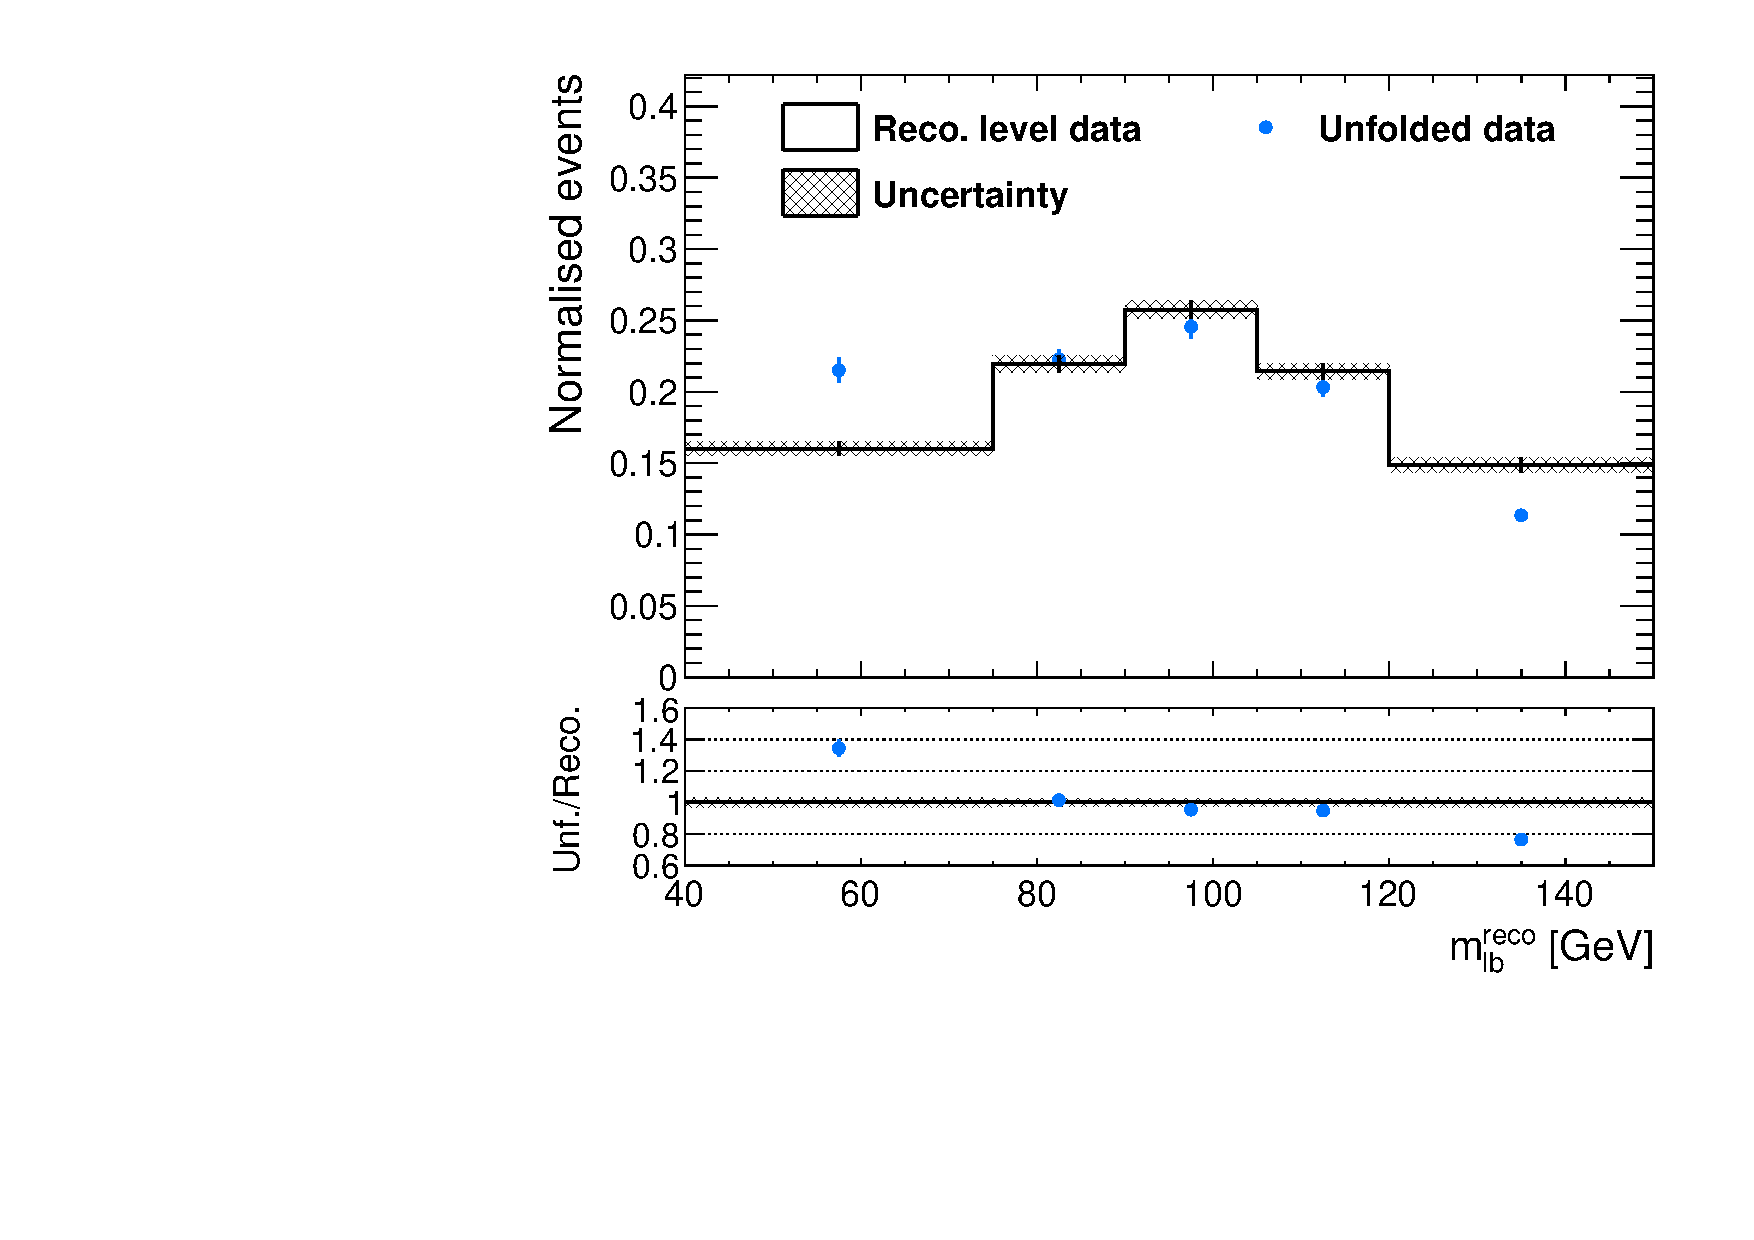
\includegraphics[width=0.7\textwidth]{./figs/fig_8TeV_TRC28_wp70_unfolding_ptlb130/mlb_unfold_hl_5bins_large_SVD_4_f1_m0_result_measunf.pdf}
  \label{sfig:unfoldeddata}
}
\hfill
\subfloat[Covariance matrix]{
  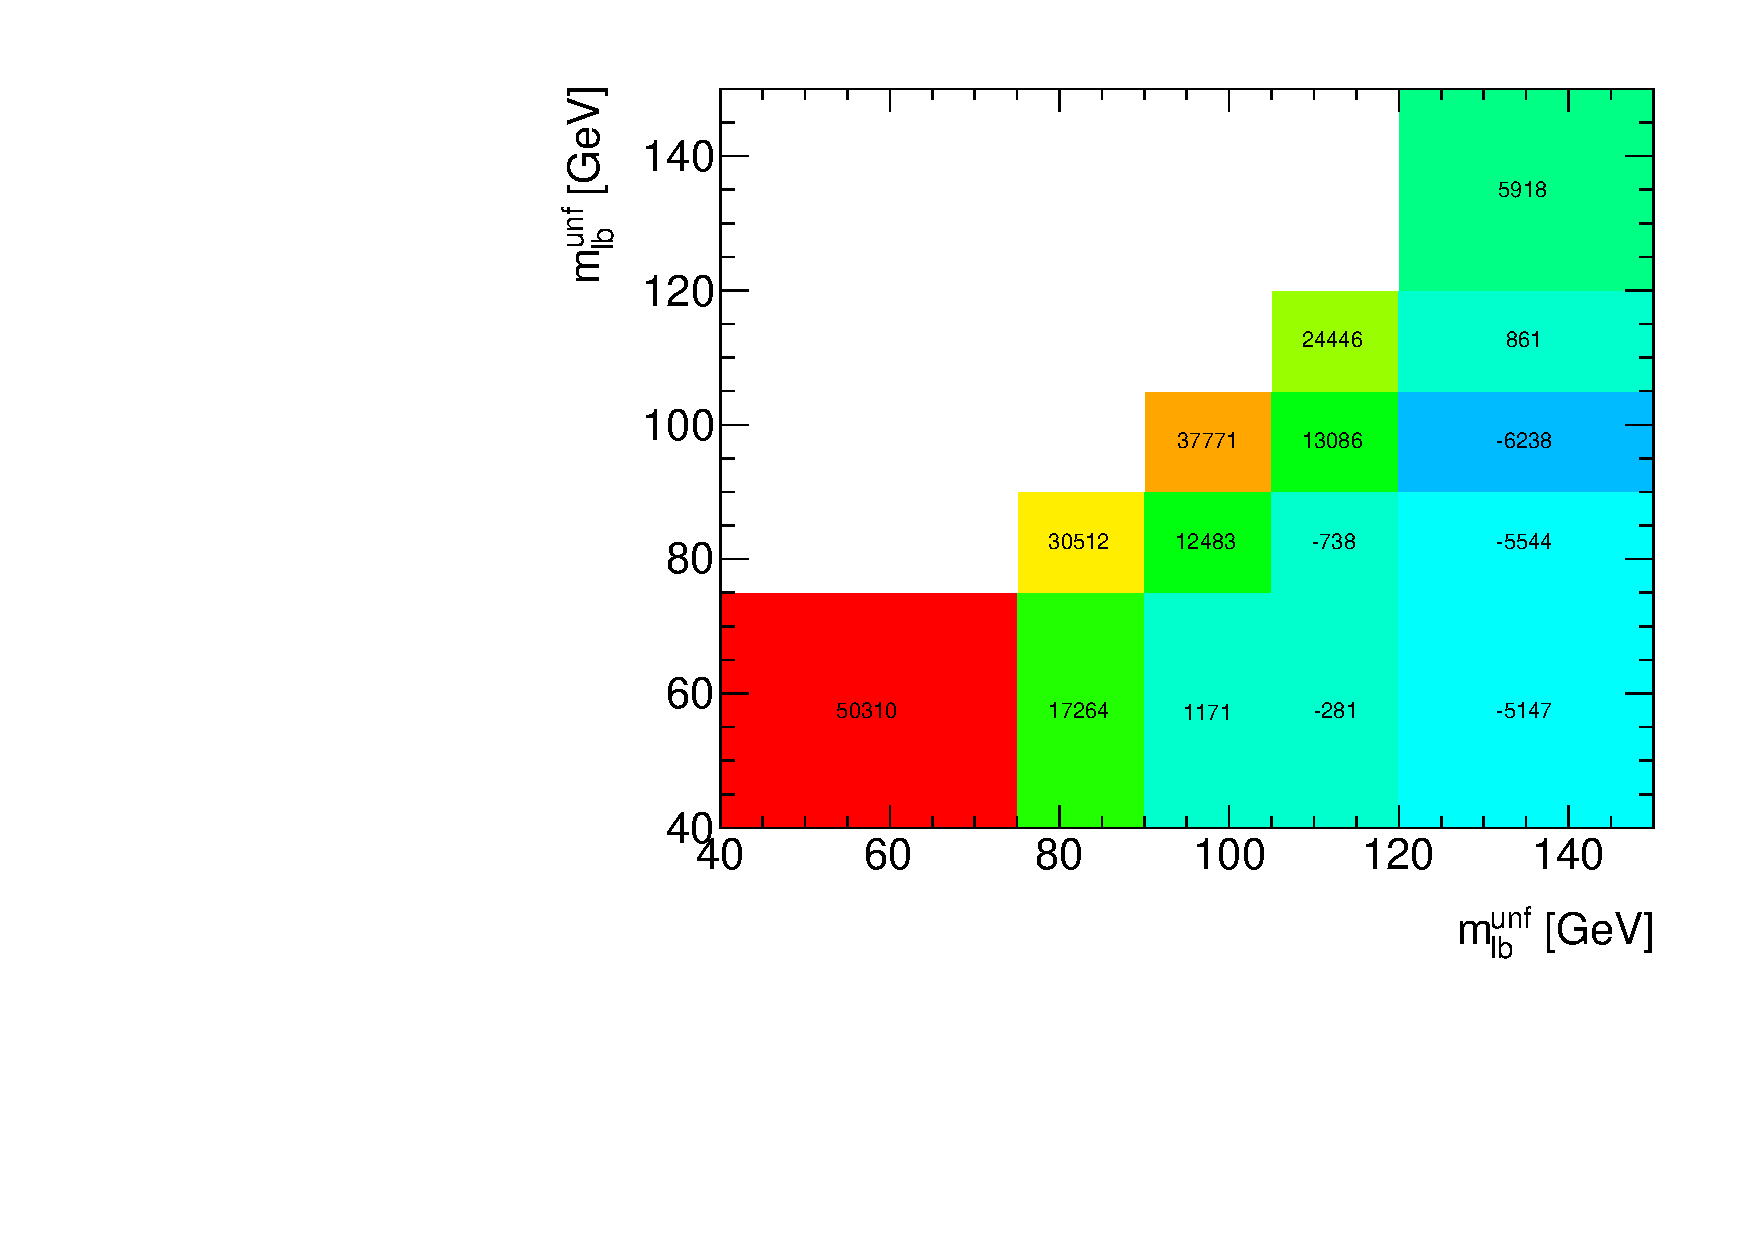
\includegraphics[width=0.7\textwidth]{./figs/fig_8TeV_TRC28_wp70_unfolding_ptlb130/mlb_unfold_hl_5bins_large_SVD_4_f1_m0_result_cov.pdf}
  \label{sfig:covariancematrixdata}
}
\caption[Unfolded \mlb\ data distribution and covariance matrix]{
%
The normalised unfolded background subtracted data \mlbr\ distribution at \truelevel\ in comparison to its original shape at \recolevel~\subref{sfig:unfoldeddata}.
%
The bins of the unfolded distribution are correlated.
%
The corresponding uncertainty band includes the uncertainties due to statistics and the unfolding procedure.
%
The bins of the \recolevel\ data are uncorrelated and the uncertainty bars are statistical only.
%
The covariance matrix corresponding to the unfolded background subtracted data distribution~\subref{sfig:covariancematrixdata}.
%
The covariance matrix consists of the variances of the independent bins in the \recolevel\ distribution and the covariances from the unfolding procedure.
%
For the symmetric matrix only one side of the diagonal is shown.
%
\label{fig:unfoldclosure}
}
\end{figure*}
%%%%%%%%%%%%%%%%%%%%%%%%%%%%%%%%%%%%%%%%%%%%%%%%%%%%%%%%%%%%%%%%%%%%%%%%%%%%%
%
%
%
%%%%%%%%%%%%%%%%%%%%%%%%%%%%%%%%%%%%%%%%%%%%%%%%%%%%%%%%%%%%%%%%%%%%%%%%%%%%%%%
\begin{figure*}[tbp!]
\centering
\subfloat[Correlation matrix]{
  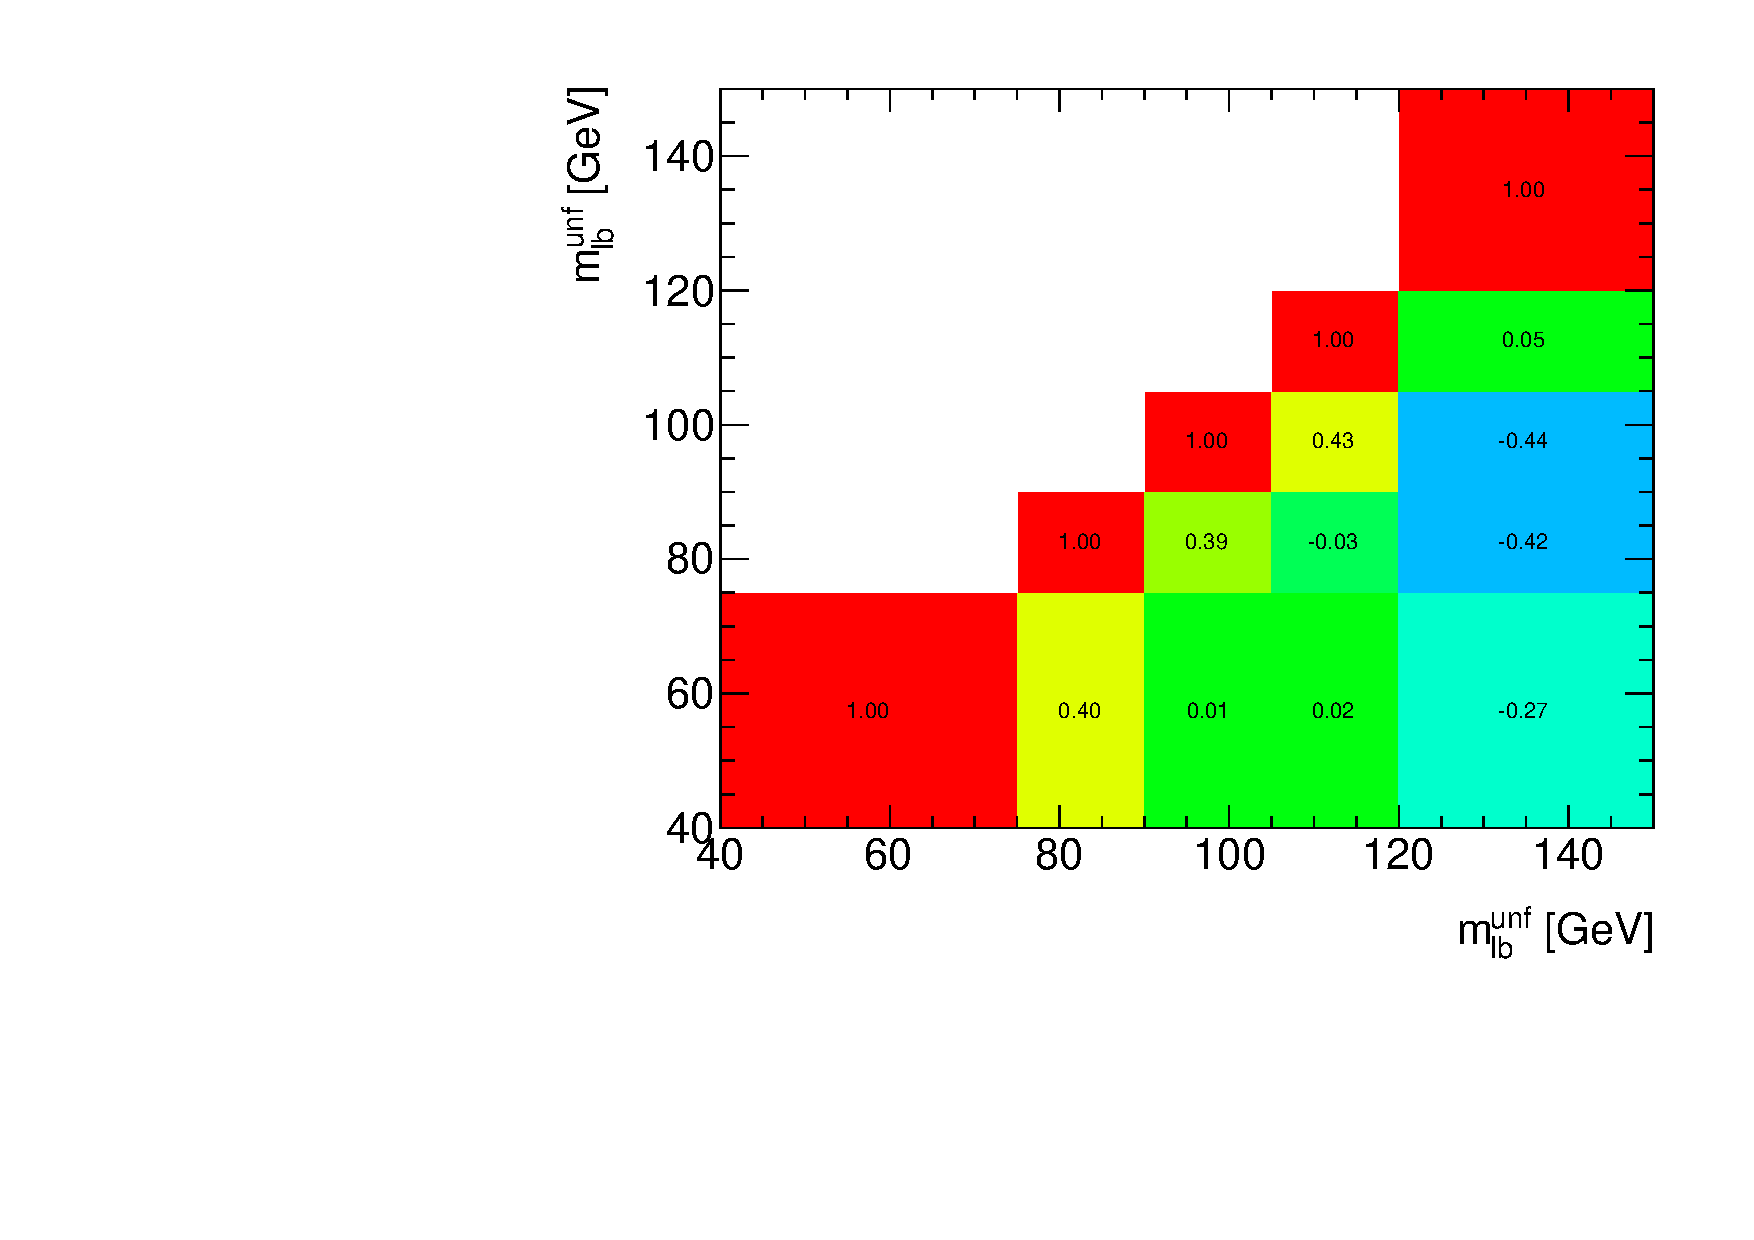
\includegraphics[width=0.7\textwidth]{./figs/fig_8TeV_TRC28_wp70_unfolding_ptlb130/mlb_unfold_hl_5bins_large_SVD_4_f1_m0_result_corr.pdf}
  \label{sfig:correlationmatrixdata}
}
\hfill
\subfloat[Unfolded data distribution and \truelevel\ templates]{
	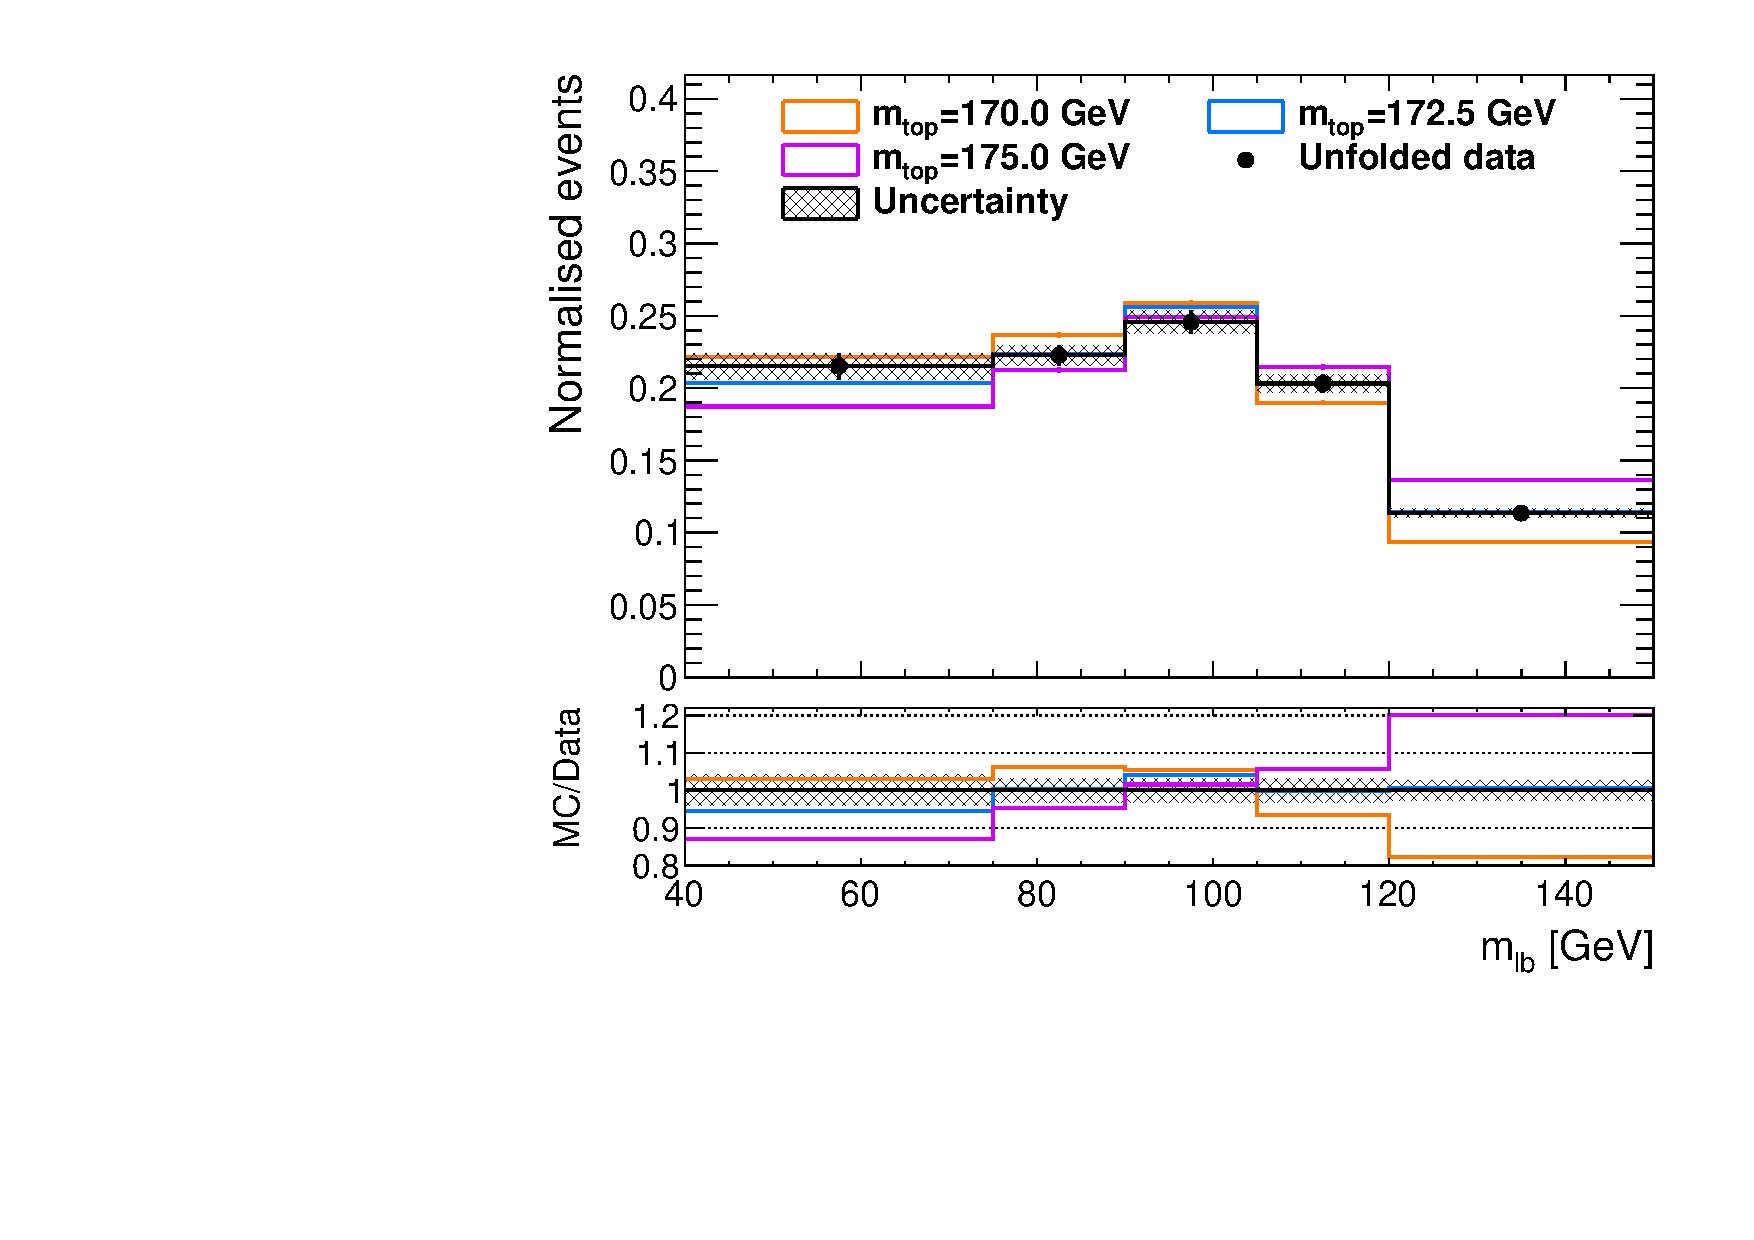
\includegraphics[width=0.7\textwidth]{./figs/fig_8TeV_TRC28_wp70_ptlb130/mlb_unfold_hl_5bins_large_SVD_4_f1_m0_Binbybin_templates.pdf}
  \label{sfig:truetemplates}
}
\caption[Correlation matrix of the unfolded \mlb\ data distribution and \truelevel\ templates]{
%
The correlation matrix corresponding to the unfolded background subtracted data distribution~\subref{sfig:correlationmatrixdata}.
%
For the symmetric matrix only one side of the diagonal is shown.
%
The normalised unfolded data distribution at \truelevel\ in comparison to the predictions at \truelevel~\subref{sfig:truetemplates}.
%
The bins of the unfolded data distribution are correlated.
%
The corresponding uncertainty band includes the uncertainties due to statistics and the unfolding procedure.
%
The bins of the \truelevel\ templates are uncorrelated and the uncertainty bars are statistical only.
%
\label{fig:unfoldclosure}
}
\end{figure*}
%%%%%%%%%%%%%%%%%%%%%%%%%%%%%%%%%%%%%%%%%%%%%%%%%%%%%%%%%%%%%%%%%%%%%%%%%%%%%


The unfolding is applied to the data distribution. The background distribution shown in \fig~\subref*{sfig:mlb_8TeV_cutbased}, this time including the single \tquark\ contribution, is subtracted from the data \mlbr\ distribution. The resulting histogram corresponds to the \ttbar\ only distribution at \recolevel. This distribution is then unfolded to obtain the underlying \mlbt\ distribution at \truelevel.
%
\Fig~\subref*{sfig:unfoldeddata} shows the resulting distribution in comparison to the background subtracted measured data distribution at \recolevel. 
%
Due to the unfolding procedure, the bins are correlated. The correlation information and individual bin uncertainties are encoded in the covariance matrix in \fig~\subref*{sfig:covariancematrixdata}. 
%
% The matrix is obtained from 1000 pseudo-experiments by varying the \recolevel\ \mlbr\ distribution within statistical uncertainties and performing the subsequent unfolding. 
%
It incorporates the statistical uncertainty on the measured data distribution and the uncertainty corresponding the inverted response matrix alike.
%
Dividing each covariance matrix element by the product of the corresponding bin uncertainties yields the correlation matrix in \fig~\subref*{sfig:correlationmatrixdata}. The matrix shows positive correlation between the first four neighbouring bins and no or negative correlation for the last bin. 
%
% This is expected from \fig~\subref*{sfig:truetemplates}.
%

The data distribution is compared to the \truelevel\ distributions of the templates for different \mt\ values. \Fig~\subref*{sfig:truetemplates} shows the template distributions, satisfying the \truelevel\ event selection specified in \sect~\ref{sect:fidphasespace}, in comparison to the unfolded data distribution. The data points lie closest to the central curve with $\mt=172.5$~\GeV. However, due to the non-diagonal covariance matrix, the naive comparison by eye can be misleading. A measurement has to be performed, taking into account the correlation of the bins.












\section{A fit with correlated histogram bins}
\label{sect:unffit}
%
From the unfolded data distribution, a measurement of \mt\ can be performed with a fit of the \truelevel\ prediction, represented by a suitable parametrisation of the \truelevel\ \gls{MC} templates. 
%
Following the approach used in \reference~\cite{ATLAS:2014zza}, the parametrisation is performed per bin using normalised distributions, interpolating the template bin contents as functions of \mt. A third order polynomial is used for the fit to the bin contents. These predictions are then used in a least-squares method to assess the optimal value of \mt. The \chiq\ to be minimised taking into account the normalised covariance matrix~\cite{CowanBook} is
%
\[
\chiq(\mt)=\sum^N_{i,j=1} (y_i-f_i(\mt)) \mathbf{V}^{-1} (y_j-f_j(\mt)).
\]
%
The indices $i$ and $j$ denote the bins with the unfolded bin contents $y$. The matrix $\mathbf{V}^{-1}$ is the inverted covariance matrix and the function $f_i$ represents the prediction for the respective bin at \truelevel. Due to the normalisation requirement, the least sensitive bin is omitted in the \chiq\ expression. For this, the first bin is chosen, because its omission deteriorates the statistical precision the least. 
%
The obtained central value is stable within uncertainties with respect to the choice of the omitted bin. 
%
The covariance matrix is normalised via a division by the square of the data distribution integral. After the inversion, the elements corresponding to the omitted bin are set to zero.
%
The statistical uncertainty is determined from the \mt\ shifts corresponding to $\Delta\chiq=+1$ around the \chiq\ minimum.






















\section{Performance of the fit}
\label{sect:unfoldsyst}
%
Before applying the method to the data or determining systematic uncertainties, the performance of the fit method and the unfolding procedure is assessed using pseudo-experiments. This is done following the same approach as the \recolevel\ analyses with a set of 1000 data-sized pseudo-experiments, randomly altering the \recolevel\ templates within their statistical uncertainty. The altered distributions are then unfolded and the fit method, calibrated with the \truelevel\ templates, is applied to assess the corresponding \mt\ value and its uncertainty.
%
%%%%%%%%%%%%%%%%%%%%%%%%%%%%%%%%%%%%%%%%%%%%%%%%%%%%%%%%%%%%%%%%%%%%%%%%%%%%%%%%%%%%%%
\begin{figure*}[tbp!]
\centering
\subfloat[\mt\ residual]{
  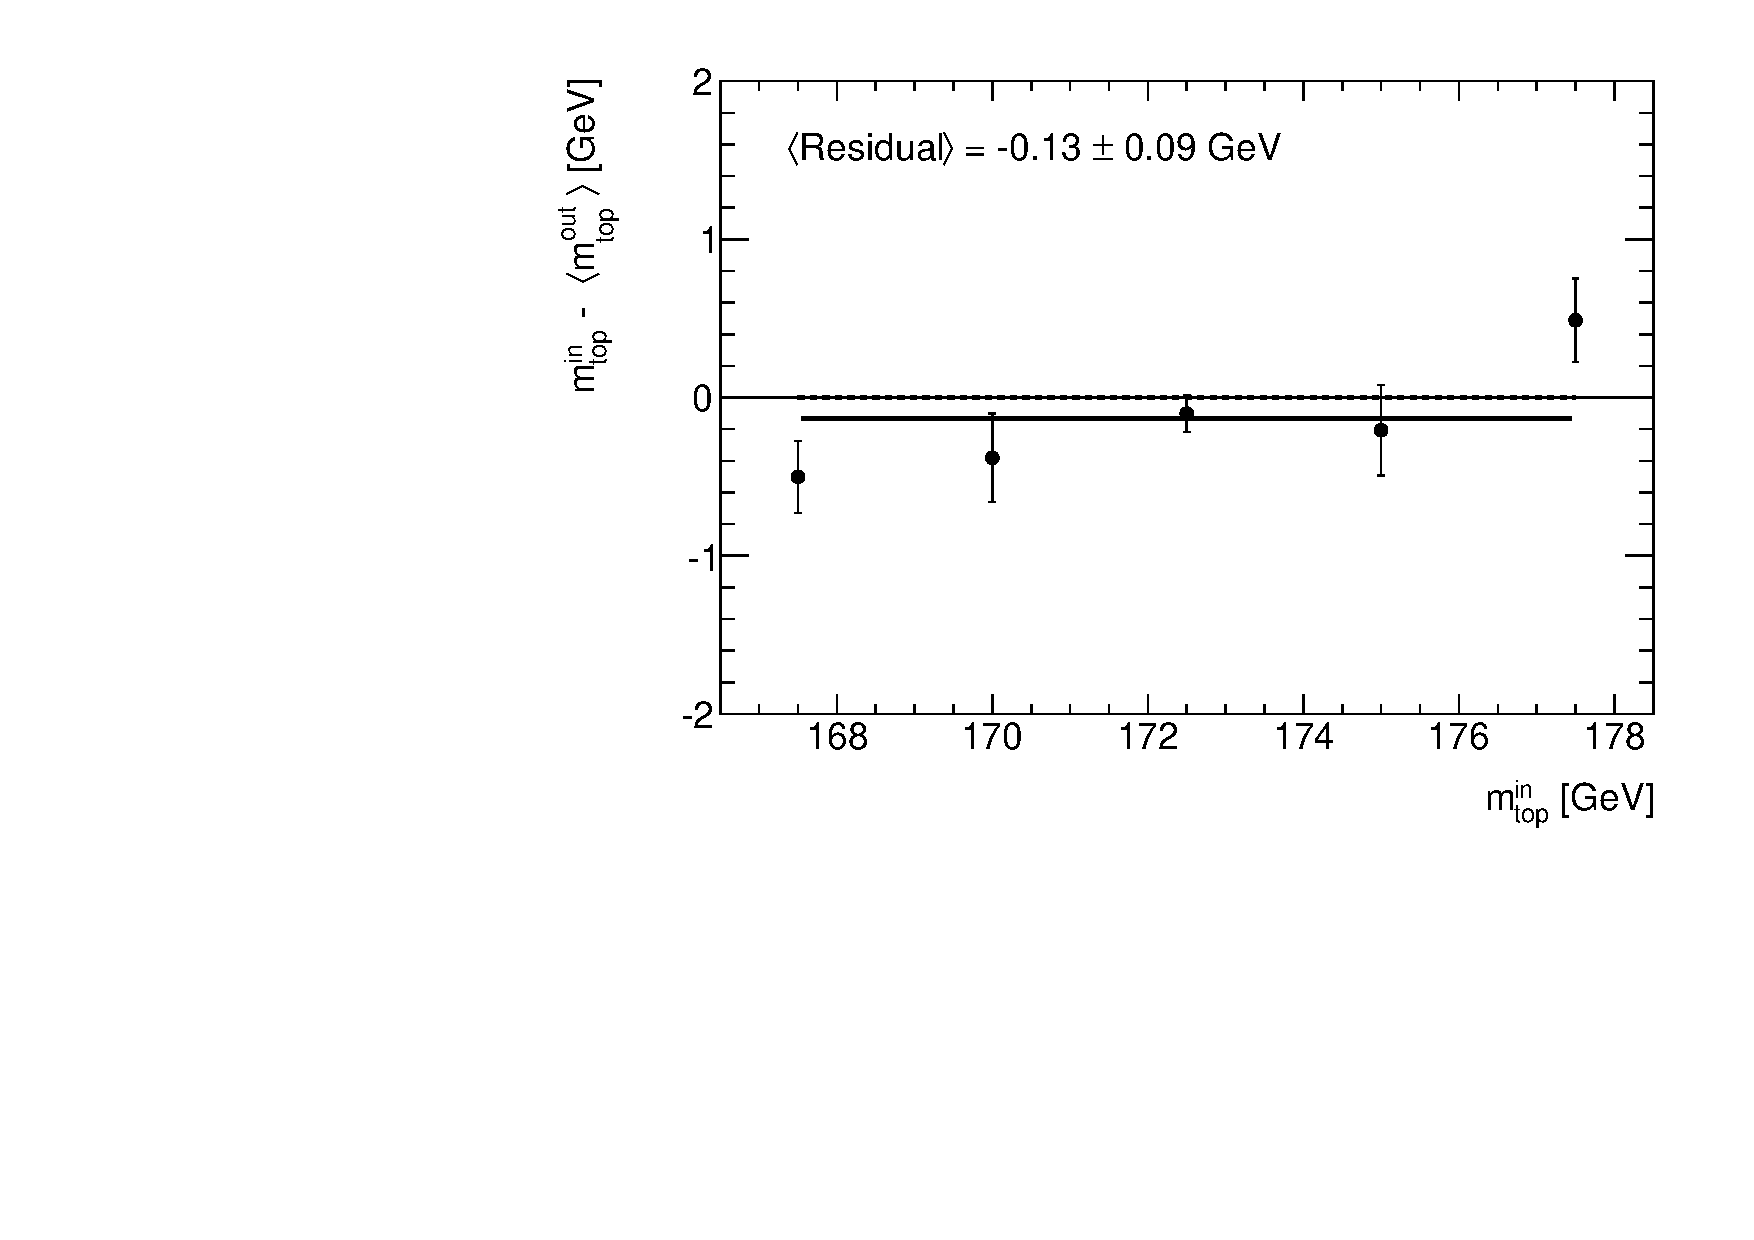
\includegraphics[width=0.49\textwidth]{./figs/fig_8TeV_TRC28_wp70_ptlb130/mlb_unfold_hl_5bins_large_SVD_4_Pexp_pe1000_invpb20277_seed0_sel3_custom12_option3_err3_massdiff.pdf}
  \label{sfig:mtopbiasunfolding}
}
\subfloat[Pull width]{
  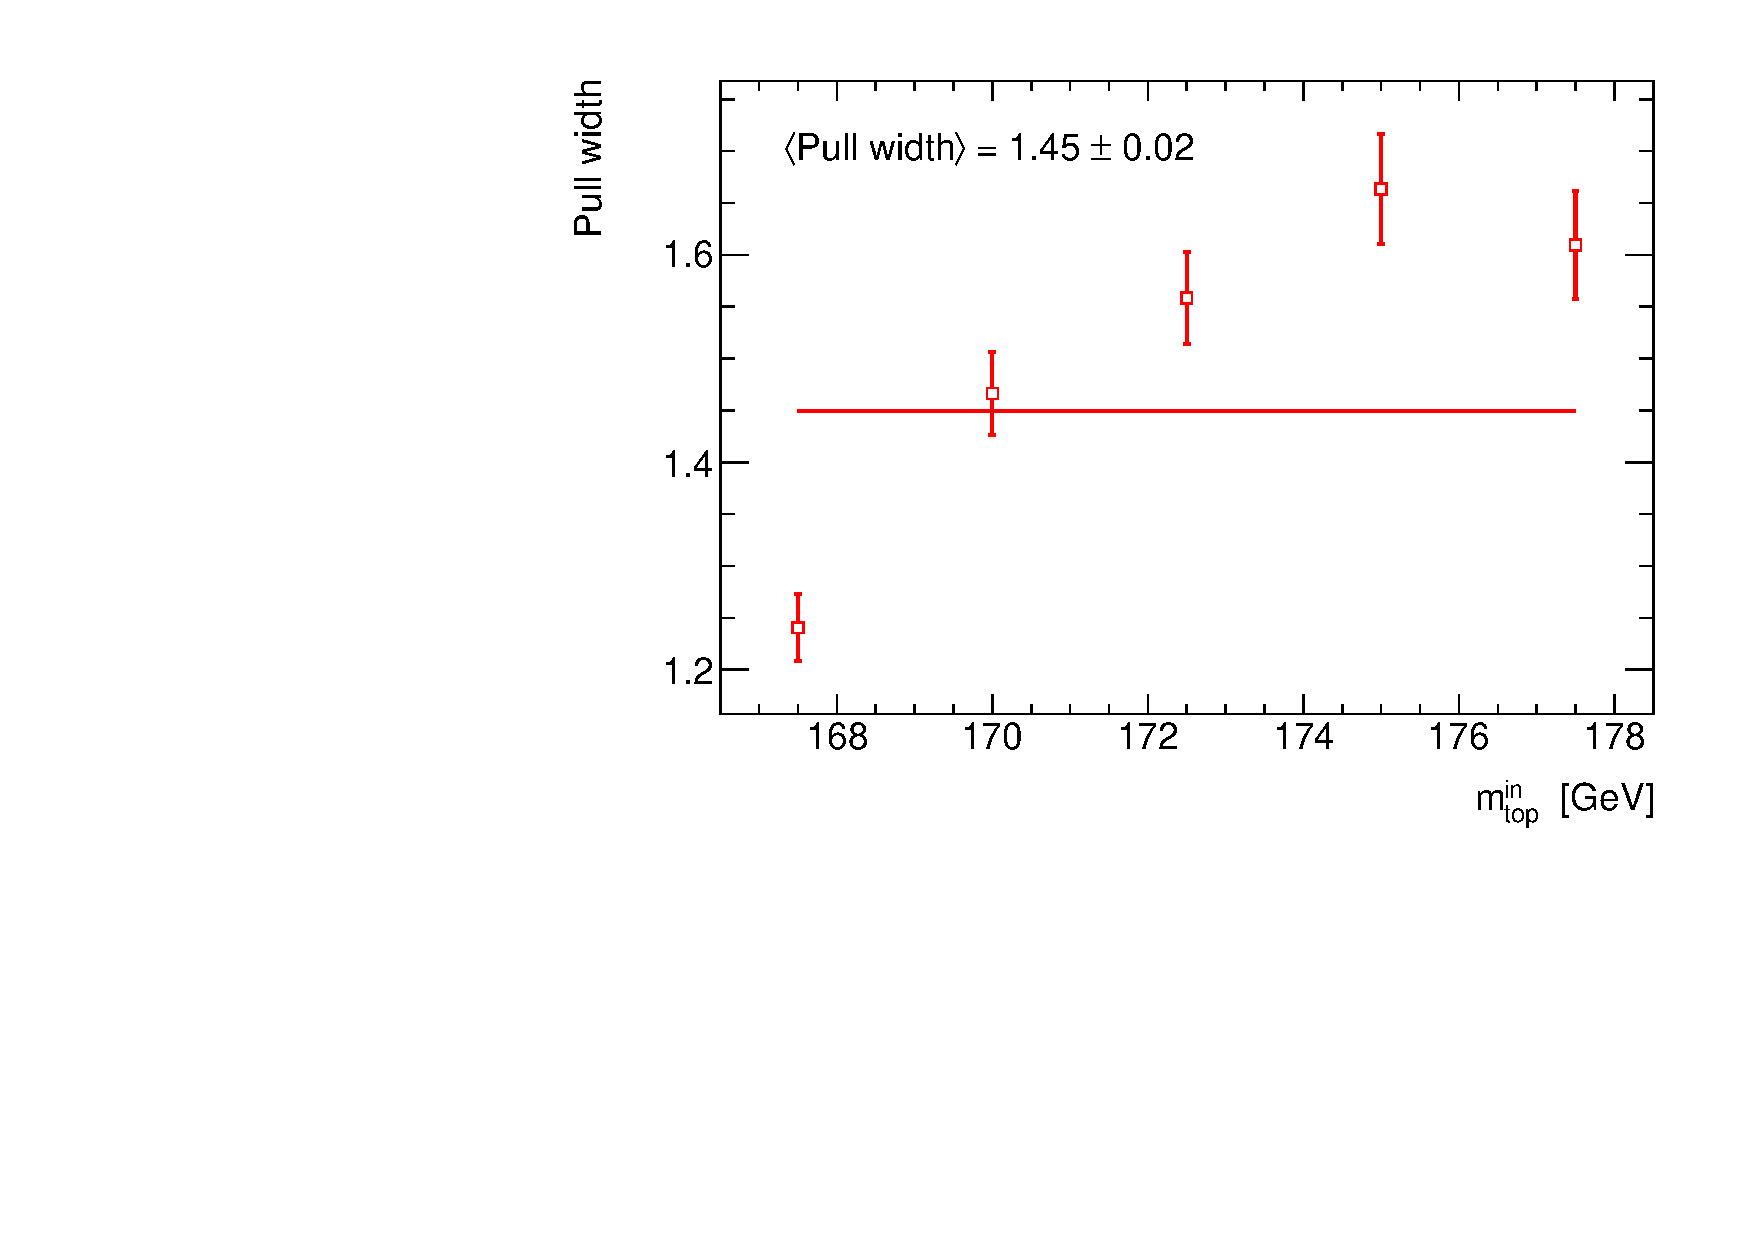
\includegraphics[width=0.49\textwidth]{./figs/fig_8TeV_TRC28_wp70_ptlb130/mlb_unfold_hl_5bins_large_SVD_4_Pexp_pe1000_invpb20277_seed0_sel3_custom12_option3_err3_pull_width.pdf}
  \label{sfig:pullwidthunfolding}
}
\caption[\mt\ residuals and pull widths for the unfolded $\sqrts=8$~\TeV\ data]{
%
\Fig~\subref{sfig:mtopbiasunfolding} shows the \mt\ residuals observed when applying the method to the respective unfolded input templates.
%
The dashed line correspond to the expected value of zero. 
%
\Fig~\subref{sfig:pullwidthunfolding} shows the pull distribution width.
%
The full lines are the result of a fit of a constant to the points. 
%
\label{fig:pullsunfolding}
}
\end{figure*}
%%%%%%%%%%%%%%%%%%%%%%%%%%%%%%%%%%%%%%%%%%%%%%%%%%%%%%%%%%%%%%%%%%%%%%%%%%%%%%%%%%%%%%
%
The resulting \mt\ residual and pull width distributions are shown in \fig~\ref{fig:pullsunfolding}.
%
The \mt\ residuals are consistent with zero. The curve exhibits a slight slope but it proves that within uncertainties, the full method, including the unfolding and the fit procedure, is not dependent on \mt\ and returns consistent central values.
%
However, the pull width distribution shows a significant trend with \mt\ and a sizeable deviation from unity. A unit pull width is expected for a method with consistent determination of statistical uncertainties. The pull width value of \UnfStatScaleFac\ for $\mtin=172.5$~\GeV\ indicates that the statistical uncertainties returned by the fit underestimate the actual fluctuation of \mt\ by this factor in the case of a fit result of $\mtout=172.5$~\GeV.
%
%%%%%%%%%%%%%%%%%%%%%%%%%%%%%%%%%%%%%%%%%%%%%%%%%%%%%%%%%%%%%%%%%%%%%%%%%%%%%%%
\begin{figure*}[tbp!]
\centering
\subfloat[Parametrisation of the first bin]{
	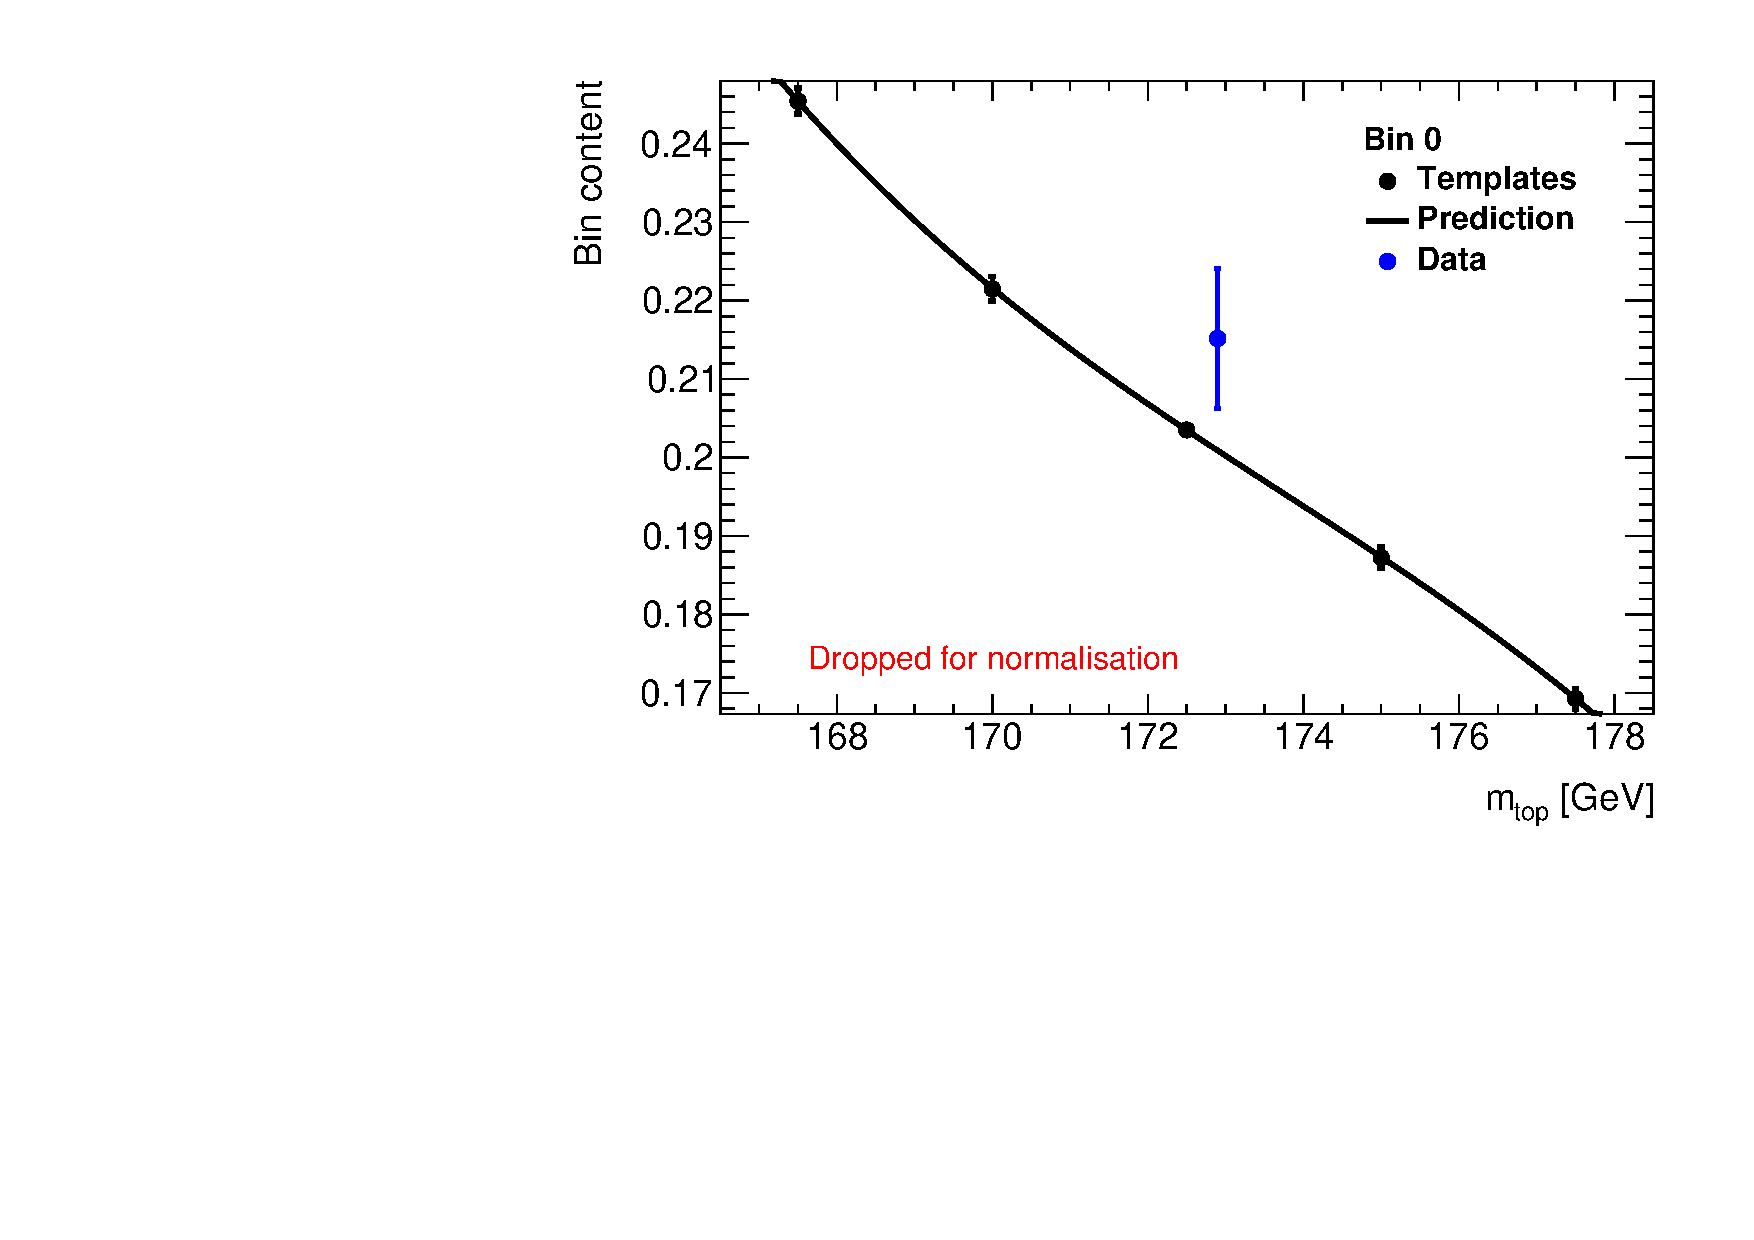
\includegraphics[width=0.49\textwidth]{./figs/fig_8TeV_TRC28_wp70_ptlb130/mlb_unfold_hl_5bins_large_SVD_4_f1_m0_param_bin0.pdf}
  \label{sfig:bin0}
}
\subfloat[Parametrisation of the second bin]{
	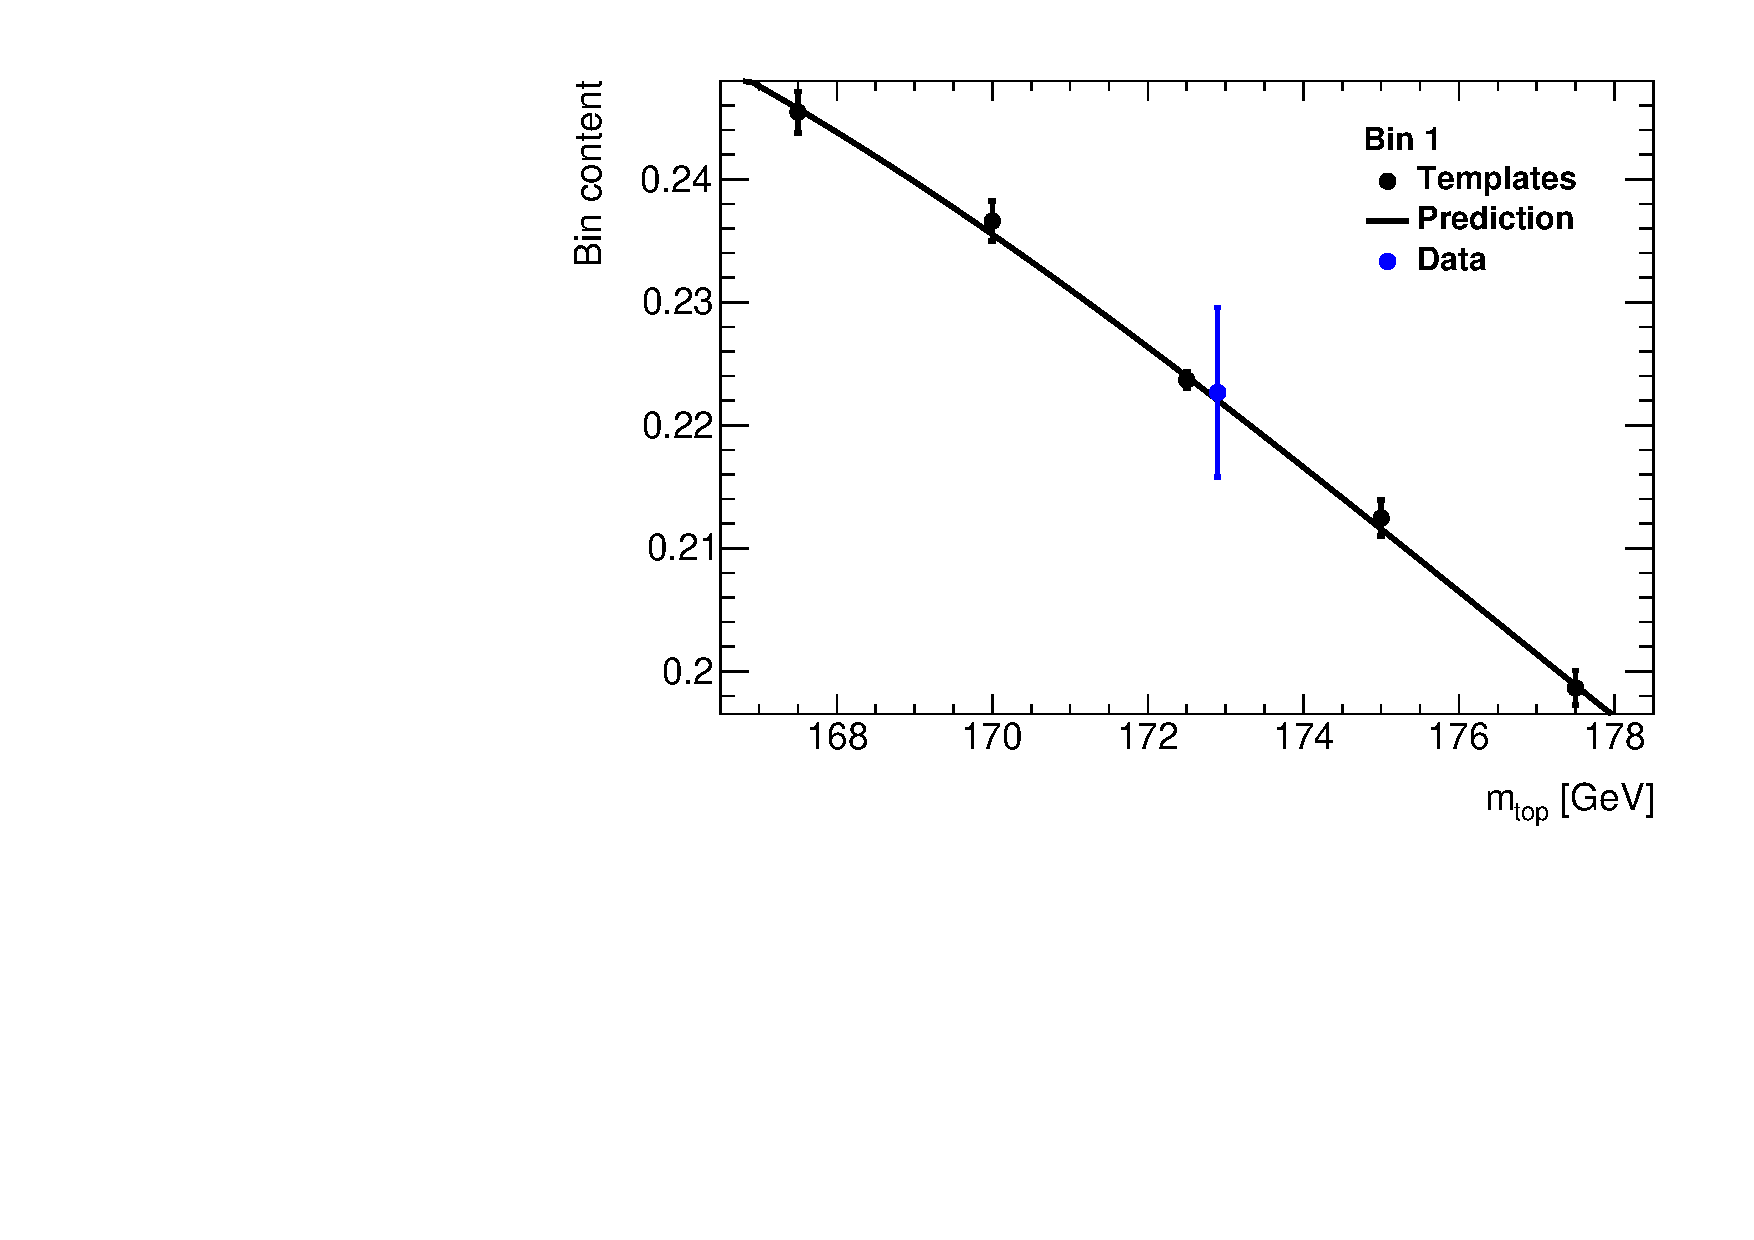
\includegraphics[width=0.49\textwidth]{./figs/fig_8TeV_TRC28_wp70_ptlb130/mlb_unfold_hl_5bins_large_SVD_4_f1_m0_param_bin1.pdf}
  \label{sfig:bin1}
}
\hfill
\subfloat[Parametrisation of the third bin]{
	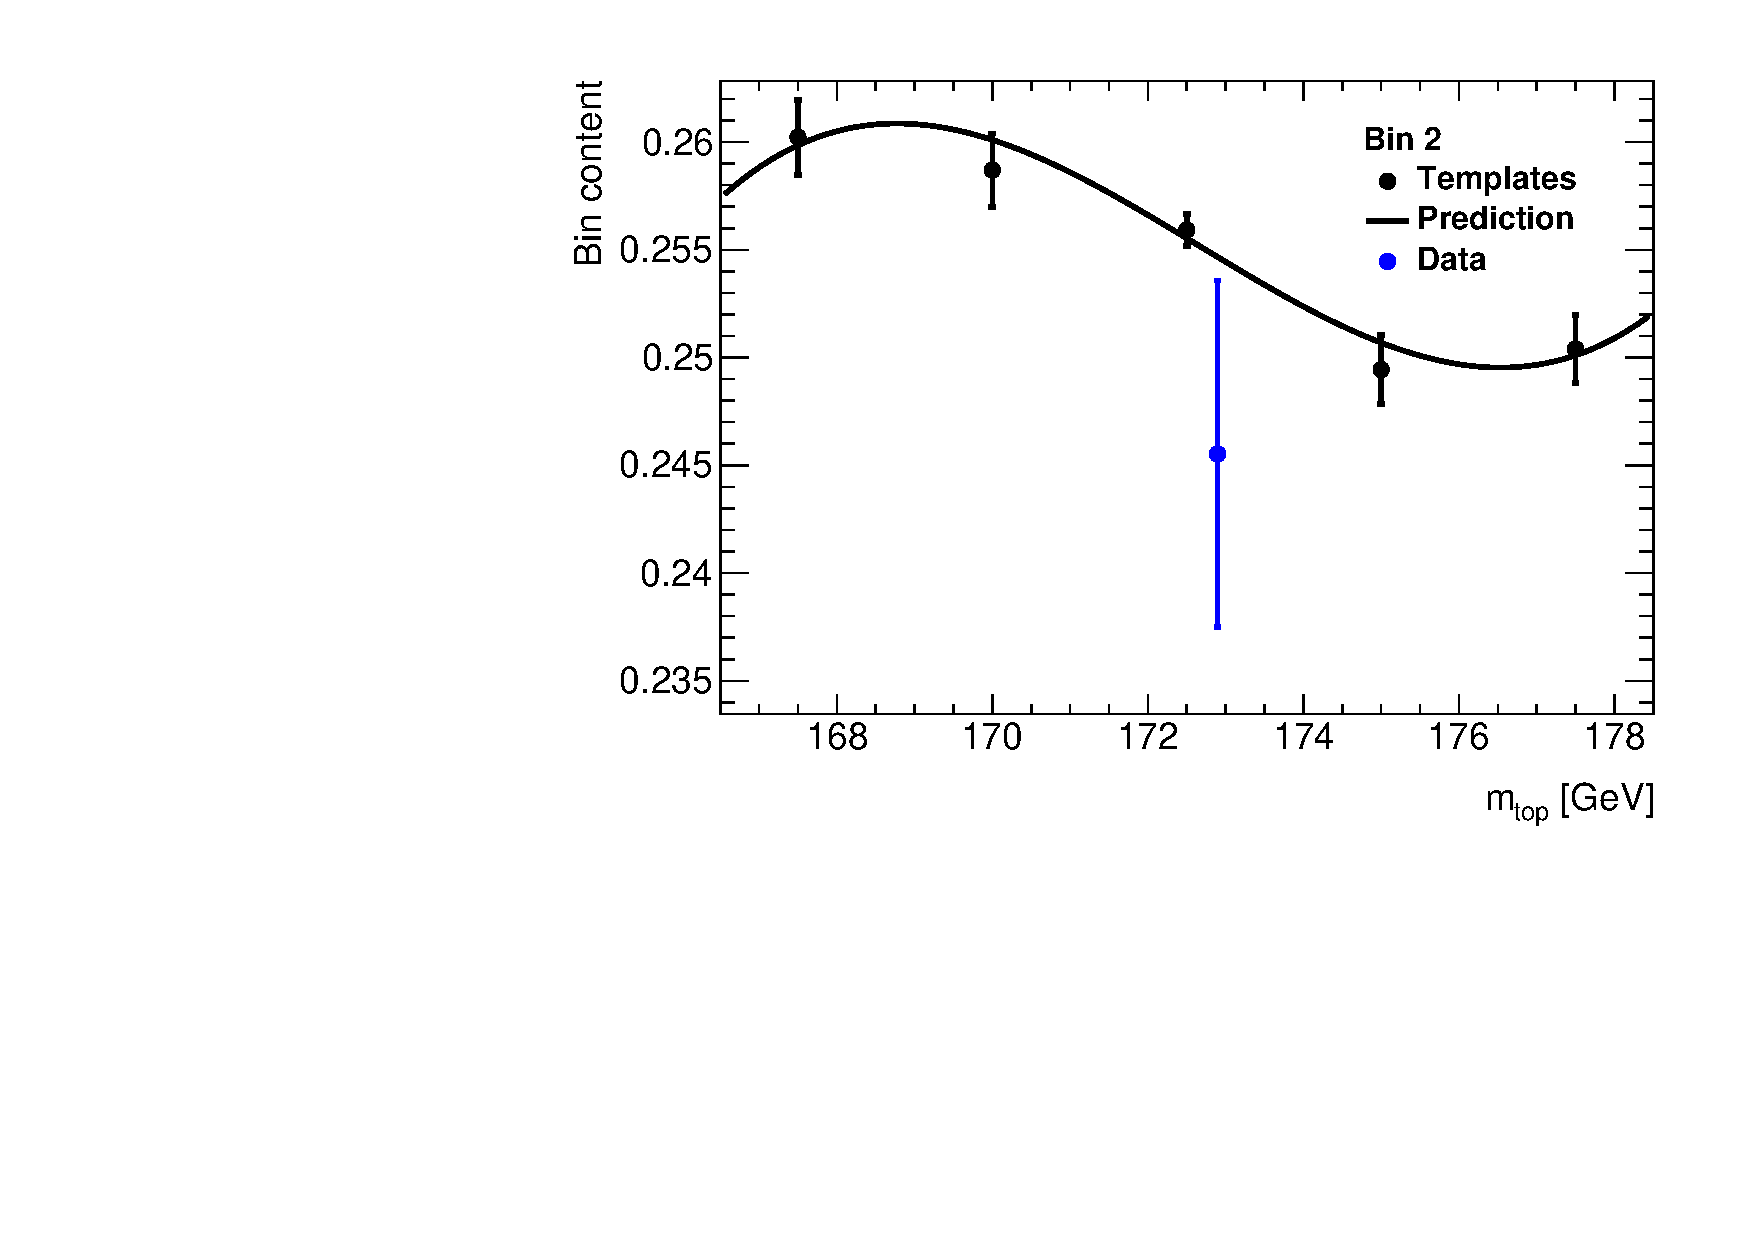
\includegraphics[width=0.49\textwidth]{./figs/fig_8TeV_TRC28_wp70_ptlb130/mlb_unfold_hl_5bins_large_SVD_4_f1_m0_param_bin2.pdf}
  \label{sfig:bin2}
}
\subfloat[Parametrisation of the fourth bin]{
	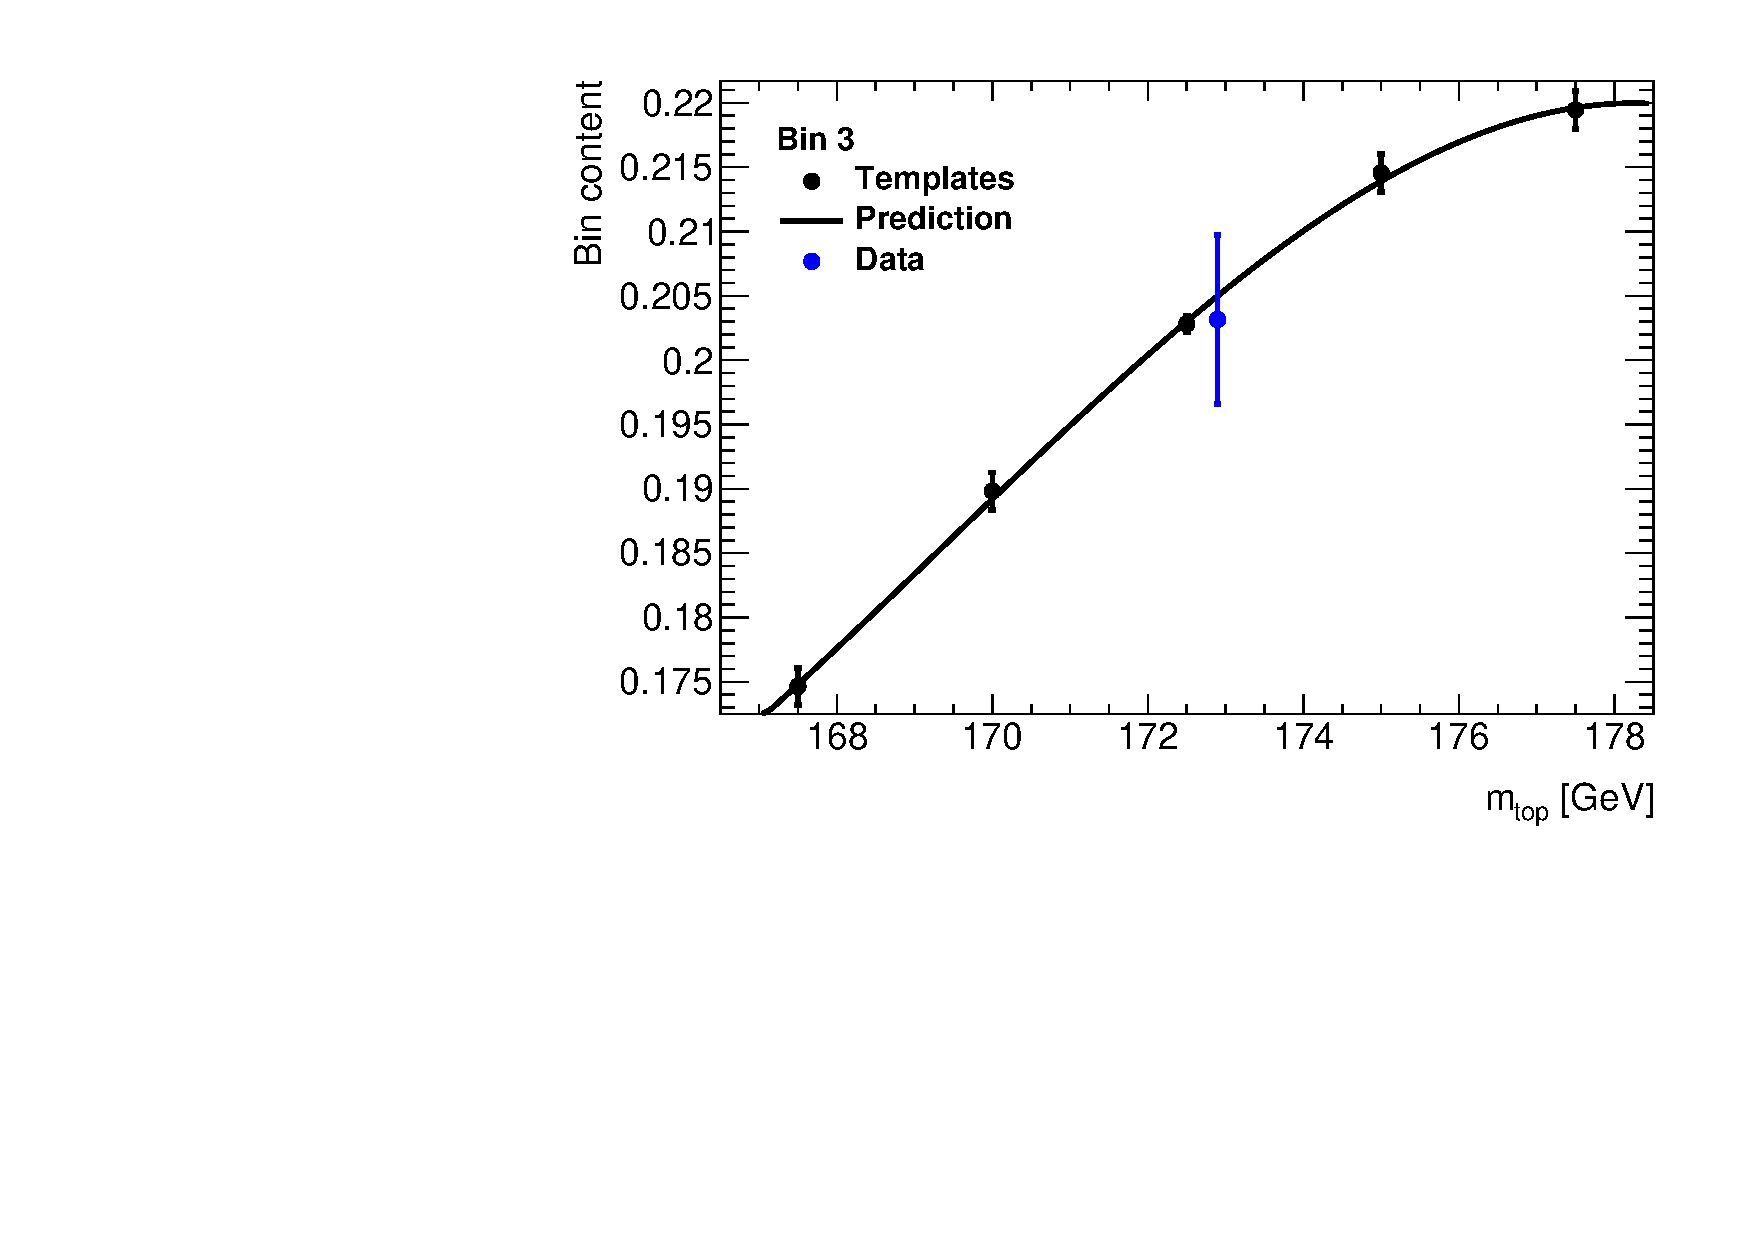
\includegraphics[width=0.49\textwidth]{./figs/fig_8TeV_TRC28_wp70_ptlb130/mlb_unfold_hl_5bins_large_SVD_4_f1_m0_param_bin3.pdf}
  \label{sfig:bin3}
}
\hfill
\subfloat[Parametrisation of the fifth bin]{
	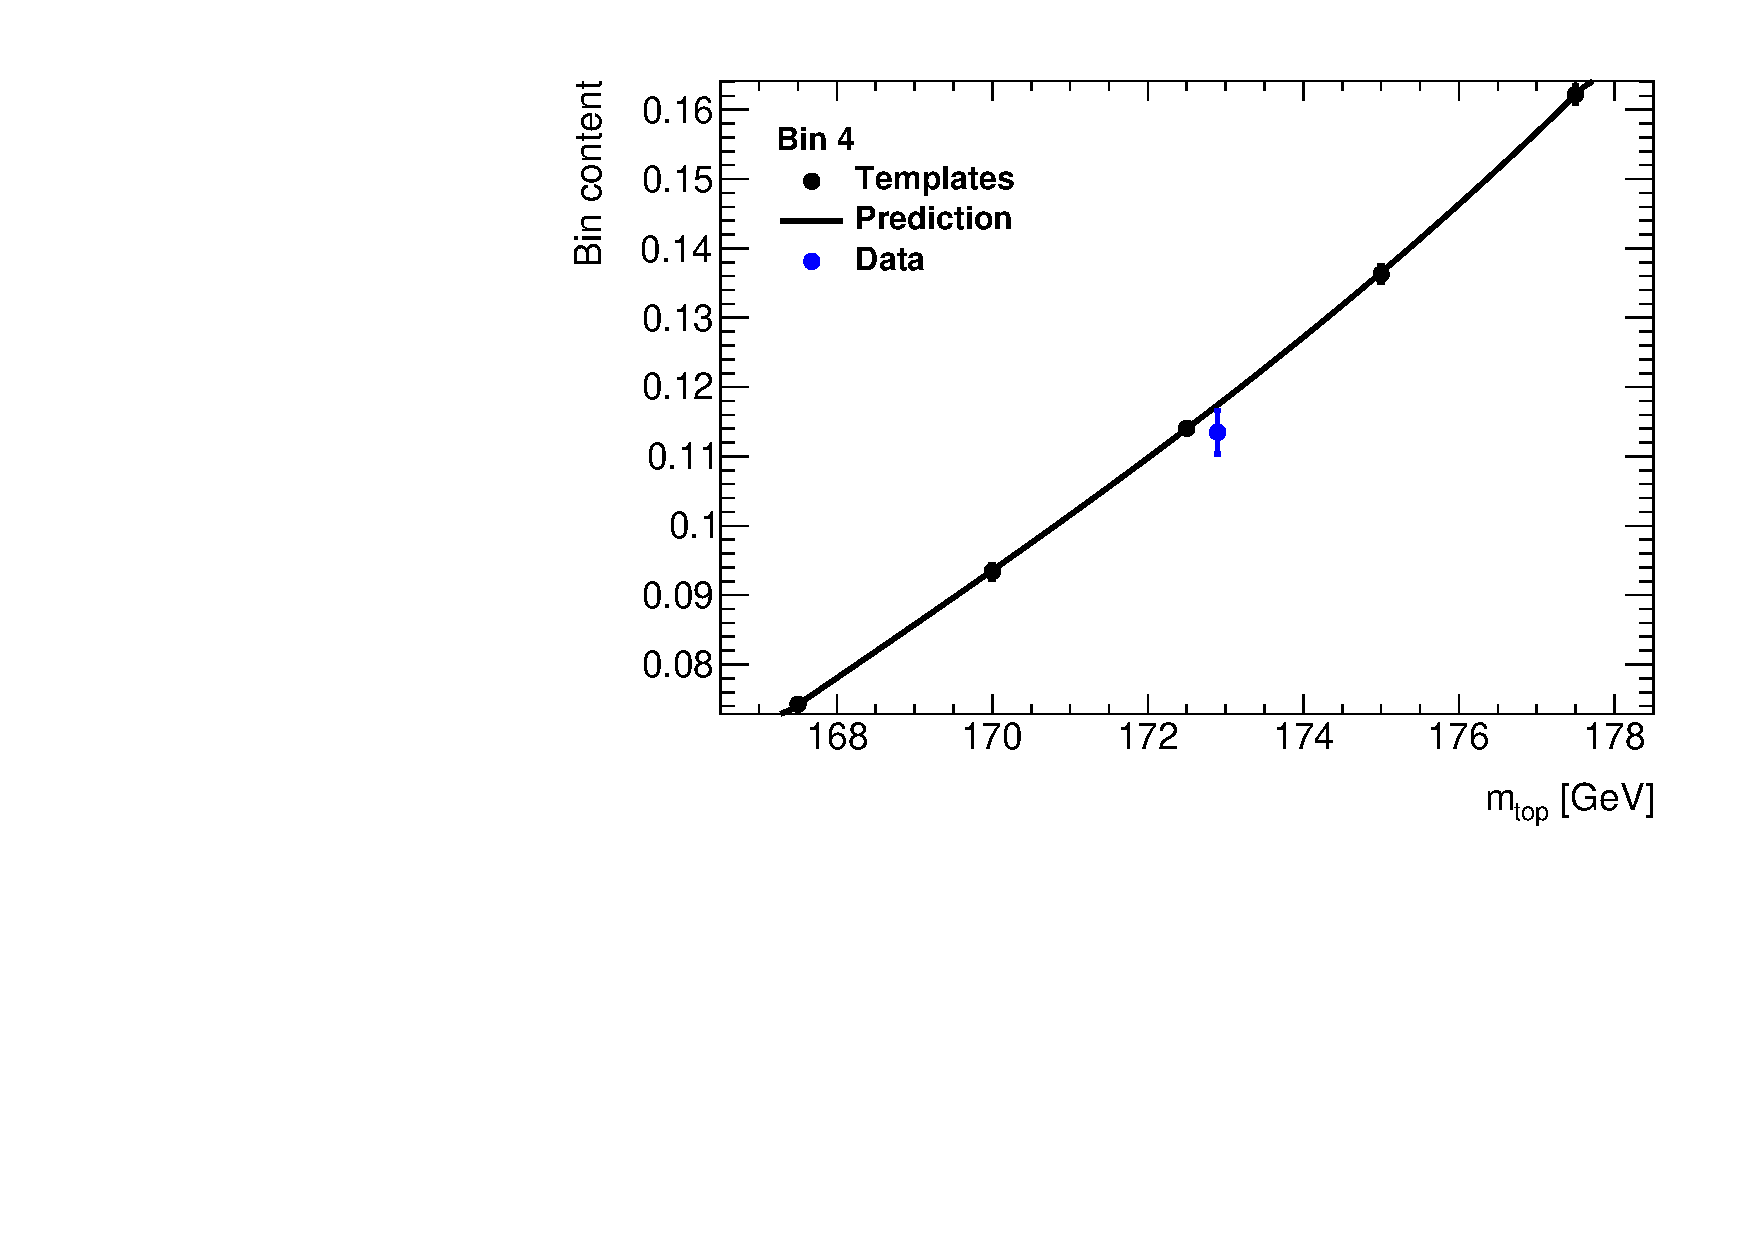
\includegraphics[width=0.49\textwidth]{./figs/fig_8TeV_TRC28_wp70_ptlb130/mlb_unfold_hl_5bins_large_SVD_4_f1_m0_param_bin4.pdf}
  \label{sfig:bin4}
}
\subfloat[The parabolic \chiq\ function]{
	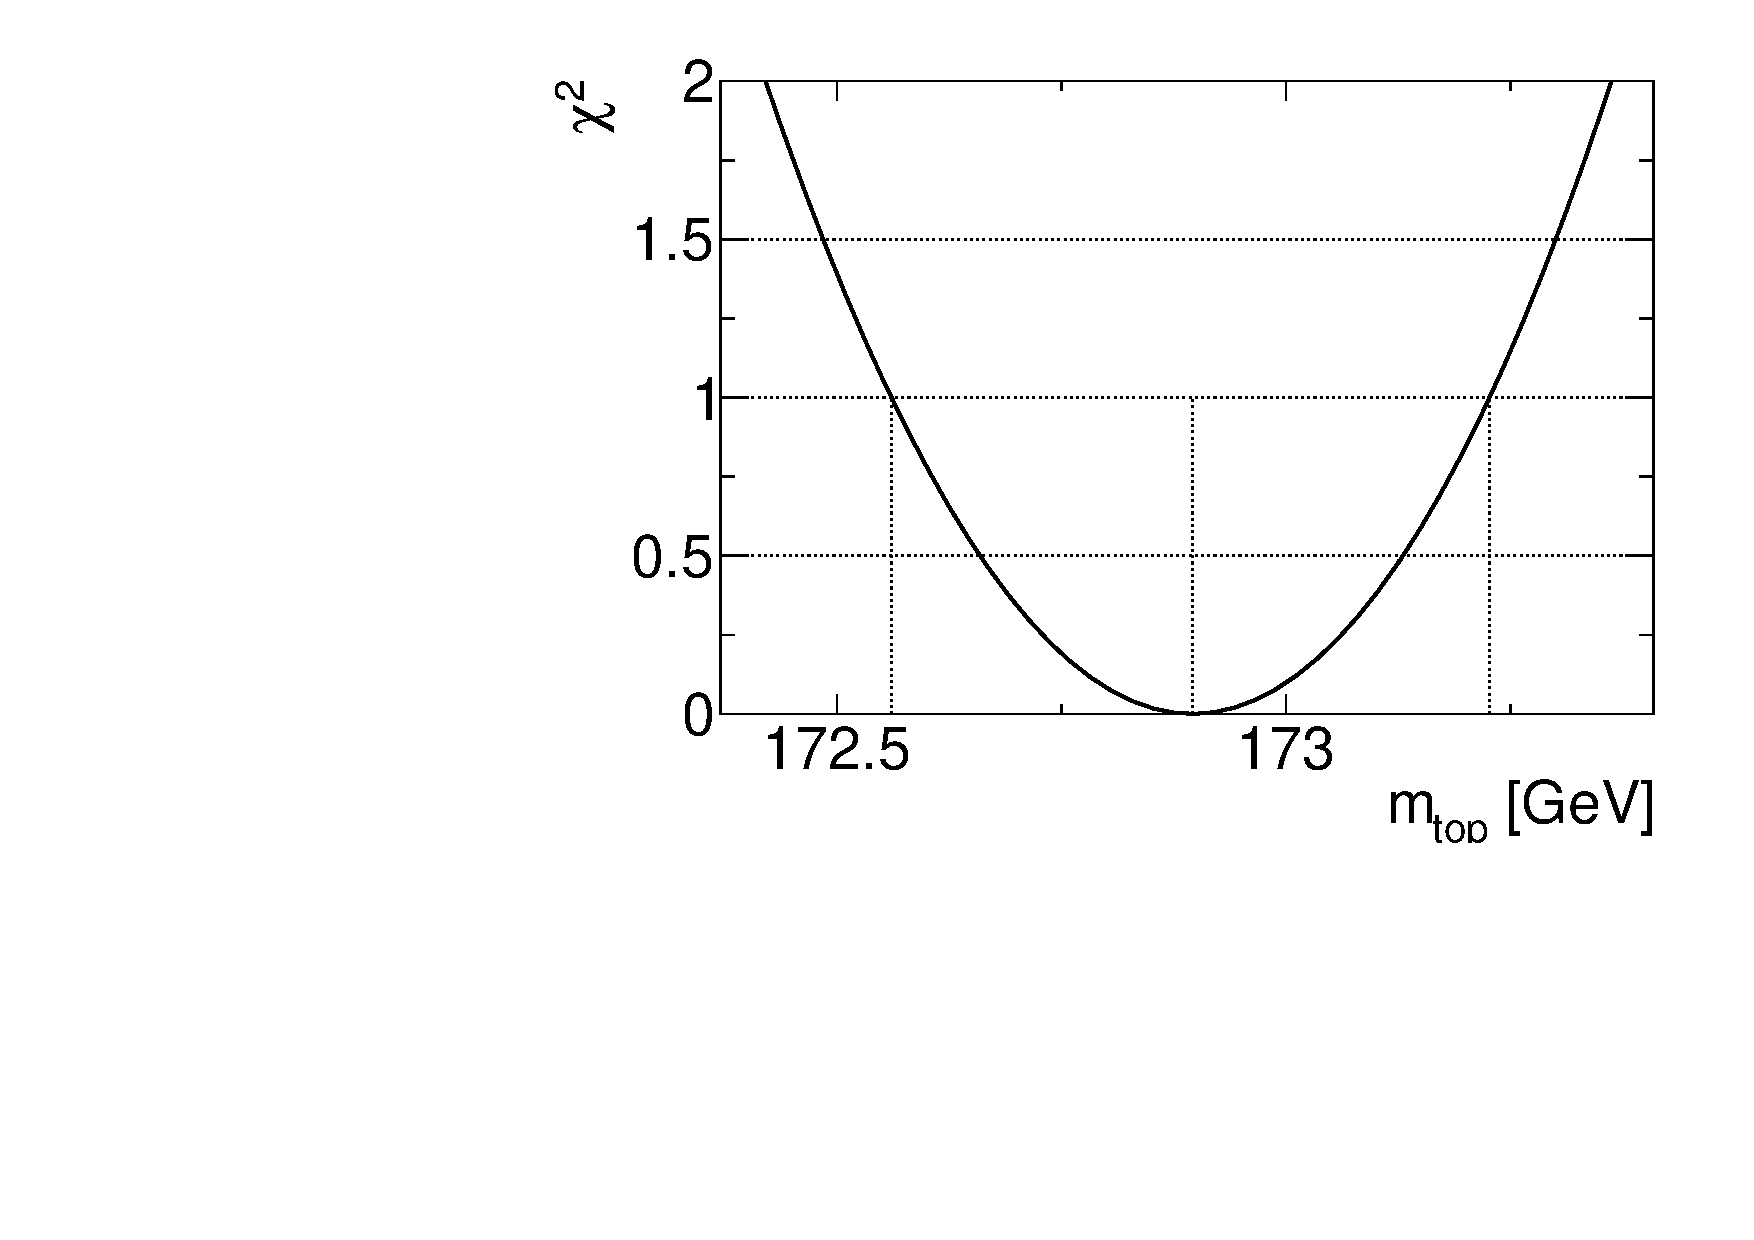
\includegraphics[width=0.49\textwidth]{./figs/fig_8TeV_TRC28_wp70_ptlb130/mlb_unfold_hl_5bins_large_SVD_4_f1_m0_Binbybin_like.pdf}
  \label{sfig:unfoldfitchi2}
}
\caption[\chiq\ fit to the unfolded distribution]{
%
\Fig{s}~\subref{sfig:bin0} to \subref{sfig:bin4} show the \truelevel\ template and unfolded data bin contents of the \mlb\ distribution. 
%
The third order polynomial parametrisation as a function of \mt\ is shown as well.
%
The data bin contents are placed at \mt-positions corresponding to the minimum of the \chiq\ distribution, shown in \fig~\subref{sfig:unfoldfitchi2}.
%
It is evaluated taking into account the bin correlations. The \mt-axis and, correspondingly, the minimum position are blinded by a constant but unknown shift.
%
\label{fig:unfoldfit}
}
\end{figure*}
%%%%%%%%%%%%%%%%%%%%%%%%%%%%%%%%%%%%%%%%%%%%%%%%%%%%%%%%%%%%%%%%%%%%%%%%%%%%%













This unbiased method can in principle be used for a measurement by correcting the statistical uncertainty for the known offset, determined from the pseudo-experiment procedure above.
%
This is shown in \Fig{s}~\subref*{sfig:bin0} to \subref{sfig:bin4}. The template bin contents and their parametrisations as a function of \mt\ are displayed, together with the bin content of the unfolded data distribution. \Fig~\subref{sfig:unfoldfitchi2} shows the corresponding \chiq\ function and its minimum for the data distribution. 
%
The minimum position is blinded with the same blinding shift as used in \chap~\ref{chap:topmass8TeV} for the $\sqrts=8$~\TeV\ analyses. The resulting \mt\ value with the statistical uncertainty scaled by the correction factor \UnfStatScaleFac\ from the pull width determination is $\mt=\XZst{\UnfValue}{\UnfStat}~\GeV\stackrel{\mathrm{scaled}}{=}\XZst{\UnfValue}{\UnfStatScaled}~\GeV$.
%
For a comparison to the central value of $\mt=\XZst{\EightValue}{\EightStat}$~\GeV, obtained from the \cutbased\ analysis at \recolevel, the statistical uncertainty is split into a fully correlated and an uncorrelated part, stemming from the limited number of data events and the unfolding procedure, respectively.
%
The uncorrelated part is taken as the difference in quadrature of the statistical uncertainties at \recol\ and unfolded level, and amounts to \UnfStatUnfPart~\GeV. Based on this, the central values at \recol\ and unfolded level are consistent within \DiffSignUnfReco\ standard deviations.
%











To optimise the method, a large number of combinations of regularisation parameters, number of bins and bin widths have been tested. A reasonable agreement between unfolded and \truelevel\ distribution could be achieved for most of them, but the performance in the fit in terms of \mt\ residuals and pull width was found to vary strongly. 
%
The employed parameter choice corresponds to the best obtained configuration.
%
Due to the non-linearity of the matrix inversion, linear behaviour of an unfolding procedure is not expected and small parameter variations can lead to significant changes of the final result. Careful tuning and optimisation are required, until a stable and consistent configuration can be achieved.  
%
Therefore, a list of systematic uncertainties is not shown and is left for future investigations. 





\section{Outlook and future studies}
%
%efficiency
Future studies should aim at a reduction of the size of the inefficiency correction, thereby reducing the uncertainty inherent to it. This can be achieved by including additional event requirements at \truelevel, such as the \met\ and \mll\ requirements in the same lepton flavour channels, and by excluding hadronically decaying tau leptons from the \truelevel\ selection.
%dressed leptons
For a consistent treatment of jets and leptons, dressed leptons should be used for the definition of the \truelevel\ objects.
%parameter choice
Further clarification of the impact of the regularisation on the unfolding, on the covariance matrix and on the fit given a particular binning, is needed. 
%discrete regularisation parameters
Especially for distributions with low numbers of bins, the limitation of the \Roounfold\ package to discrete regularisation parameters prevents a fine tuning.
%event by event unfolding
An unfolding based on events rather than histograms, taking into account the detector effects on various variables, can be used to gain more control of the sanity of the unfolded distributions. This can potentially result in increased resolution. This is for example implemented in the \TRUEE\ program~\cite{TRUEE,Milke2013133}.







\section{Summary}
%
An approach to measure the \tquark\ mass at \stablevel\ has been outlined, using unfolded estimator distributions. The investigations constitute the first steps towards a measurement of \mt\ at \stablevel.
%
The approach allows for the determination of theoretical uncertainties and the investigation of theoretical effects without the computing intensive detector simulation, and therefore with high statistical precision. 
%
This chapter concludes the experimental part of this work.
%
% However, for a successful comparison to theory predictions, this technique requires an unambiguous definition of the \truelevel\ phase space. While this is in general not a problem for \stablevel, it is difficult to achieve for the convention-dependent \genlevel. For predictions without \gls{PS} matching, other techniques have to be employed. One of those is shown next. 
